% ---------------------------------------------------------------------
% --- Arquivo principal e os demais serao os dos capitulos.
% --- EXPRESSÔES ENTRE <> DEVERÃO SER COMPLETADAS COM A INFORMAÇÂO ESPECÍFICA DO TRABALHO 
% ---------------------------------------------------------------------

\documentclass[ruledheader]{abnt_UFF}

%==\usepackage[colorlinks]{hyperref}
%\usepackage[printonlyused,withpage]{acronym}


%--- Appendix
\usepackage[toc,page]{appendix}

%---pacotes para hiphenizacao e acentuacao em portugues
\usepackage[utf8]{inputenc}
\usepackage[brazil]{babel}
\usepackage[T1]{fontenc}


%---fornece a capacidade de criar hiperlinks no documento
%\usepackage[dvips,colorlinks=False, pdfstartview=FitV,citecolor=green,urlcolor=black,plainpages=false, pdftitle={Disserta\c{c}\~ao de Mestrado Yona Lopes}]{hyperref}%backref,
\usepackage[hidelinks, breaklinks, colorlinks=false, pdfstartview=FitV, linkcolor=black, citecolor=green,urlcolor=black,plainpages=false]{hyperref} % usar  hidelinks para esconder os links, continuara o link mas sem aparecer cor ou borda

\usepackage[breaklinks]{hyperref} % Problema quando o nome da figura/tabela/se\c{c}\~ao eh grande
%\usepackage[dvips,pdfstartview=FitV]{hyperref}%backref,
%\usepackage[dvips]{color}
	
%---pacotes para criacao de index
\usepackage{makeidx}
%\usepackage[pdftex,colorlinks=true, pdfstartview=FitV, linkcolor=black, citecolor=black,urlcolor=black,plainpages=false]{hyperref}
\usepackage{pdfcolmk}

%--- pacote para figuras
\usepackage{epsf}
\usepackage{epsfig,graphicx}
\usepackage{subfigure}


%--- pacote de simbolos
\usepackage{latexsym}
%\usepackage{textcomp}

%--- simbolos matematicos
\usepackage{amsmath}
%\usepackage{amssymb}

%----- c\'{o}digos fonte
\usepackage{listings}
% op\c{c}\~oes do pacote listings
\lstset{numbers=left, language=java, stepnumber=1, firstnumber=1, numberstyle=\tiny, extendedchars=true, breaklines=true, frame=tb, basicstyle=\footnotesize, stringstyle=\ttfamily, showstringspaces=false backgroundcolor=\color{gray}}

\newcommand\JSONnumbervaluestyle{\color{blue}}
\newcommand\JSONstringvaluestyle{\color{red}}

% switch used as state variable
\newif\ifcolonfoundonthisline

\makeatletter

\lstdefinestyle{shared}
{
	breaklines=true,
	tabsize=2,
	columns=flexible,
	morestring          = [s]{"}{"},
	stringstyle         = \ifcolonfoundonthisline\JSONstringvaluestyle\fi,
	inputencoding=utf8
}

\lstdefinestyle{json}
{
	style=shared,
	showstringspaces    = false,
	keywords            = {false,true},
	alsoletter          = 0123456789.,
	MoreSelectCharTable =%
	\lst@DefSaveDef{`:}\colon@json{\processColon@json},
	basicstyle          = \ttfamily,
	keywordstyle        = \ttfamily\bfseries,
}

\lstdefinestyle{python}
{
	style=shared,
	language={Python},
	%alsolanguage={[Sharp]C},
	basicstyle=\small\tt,
	keywordstyle=\color{blue},
	commentstyle=\color[rgb]{0.13,0.54,0.13},
}

% flip the switch if a colon is found in Pmode
\newcommand\processColon@json{%
	\colon@json%
	\ifnum\lst@mode=\lst@Pmode%
	\global\colonfoundonthislinetrue%
	\fi
}

\lst@AddToHook{Output}{%
	\ifcolonfoundonthisline%
	\ifnum\lst@mode=\lst@Pmode%
	\def\lst@thestyle{\JSONnumbervaluestyle}%
	\fi
	\fi
	%override by keyword style if a keyword is detected!
	\lsthk@DetectKeywords% 
}

% reset the switch at the end of line
\lst@AddToHook{EOL}%
{\global\colonfoundonthislinefalse}

\makeatother

% pacote para posicionamento de tabelas e figuras
\usepackage{float}
\restylefloat{table}


%--- pacote para gerar pseudo-codigo
%\usepackage{algorithm}
%\usepackage{algorithmic}
% \usepackage[linesnumbered,boxed,lined]{algorithm2e} 
\usepackage[algoruled,portuguese,linesnumbered]{algorithm2e} 
%\floatname{algorithm}{Algoritmo}

%--- outros pacotes
\usepackage{url}
\usepackage{longtable}
\usepackage{lscape}

%\usepackage[notbib, notlof, notlot]{tocbibind}

%Tabela Colorida e pacotes de tabela
%\usepackage{colortbl}
\usepackage{array}

%--- Acronyms
%\usepackage{acronym}
\usepackage[printonlyused,withpage]{acronym}

\usepackage{multicol}
\usepackage{multirow}
\usepackage{rotating}

%--- Notes
\usepackage{todonotes}

\hyphenation{
a-de-qua-da-men-te 
di-men-sio-na-men-to 
re-di-re-cio-na
}

%---------usando tipo de fonte padrao
\renewcommand{\ABNTchapterfont}{\bfseries\fontfamily{cmr}\fontseries{b}\selectfont}
\renewcommand{\ABNTsectionfont}{\bfseries\fontfamily{cmr}}

\newcommand{\todot}[1]{\todo[color=green!40,fancyline]{#1}}


\makeindex
% --- -----------------------------------------------------------------
% --- Documento Principal.
% --- -----------------------------------------------------------------
%\usepackage[pdftex]{hyperref}
%\hypersetup{colorlinks, sitecolor=black, pdftex}
\begin{document}

% --- -----------------------------------------------------------------
% --- Titulo, abstract, dedicatorias e agradecimentos.
% --- Indice geral, lista de figuras e tabelas.
% --- -----------------------------------------------------------------

% --- -----------------------------------------------------------------
% --- Elementos usados na Capa e na Folha de Rosto.
% --- EXPRESSES ENTRE <> DEVERO SER COMPLETADAS COM A INFORMAO ESPECFICA DO TRABALHO
% --- E OS SMBOLOS <> DEVEM SER RETIRADOS 
% --- -----------------------------------------------------------------
\autor{NICOLAS DE SOUSA TEODOSIO E VICTOR HUGO NOVAIS RODRIGUES} % deve ser escrito em maiusculo

\titulo{ANÁLISE DE SENTIMENTO E MINERAÇÃO DE OPINIÕES APLICADO NO TWITTER} % deve ser escrito em maiusculo

\instituicao{INSTITUTO INFNET} % deve ser escrito em maiusculo

\orientador{CASSIUS FIGUEIREDO}% deve ser escrito em maiusculo - preencher com o nome do seu orientador

%\coorientador{NOME} %preencher se houver.

\local{RIO DE JANEIRO} % deve ser escrito em maiusculo

\data{2016} % ano da defesa

\comentario{Trabalho de Conclusão de Curso apresentado ao Programa de Graduação em Engenharia da Computação do \mbox{Instituto Infnet} como parte dos requisitos necessários à obtenção do título de \mbox{Bacharel em Engenharia da Computação}.}%preencha com a sua area de concentracao


% --- -----------------------------------------------------------------
% --- Capa. (Capa externa, aquela com as letrinhas douradas)(Obrigatorio)
% --- ----------------------------------------------------------------
\capa

% --- -----------------------------------------------------------------
% --- Folha de rosto. (Obrigatorio)
% --- ----------------------------------------------------------------
\folhaderosto


\pagestyle{ruledheader}
\setcounter{page}{1}
\pagenumbering{roman}

% --- -----------------------------------------------------------------
% --- Ficha Catalográfica. (Obrigatorio)
% --- ----------------------------------------------------------------
%
%\cleardoublepage
%\thispagestyle{empty}
%\vspace*{130mm}
%
%\begin{flushright}
%
%\hspace{8em}
%\fbox{\begin{minipage}{10cm}

%....

%\end{minipage}}
%
%\end{flushright}
%\newpage

% --- -----------------------------------------------------------------
% --- Termo de aprovacao. (Obrigatorio)
% --- ----------------------------------------------------------------


\cleardoublepage
\thispagestyle{empty}

\vspace{-60mm}

\begin{center}
   {\large NICOLAS DE SOUSA TEODOSIO E VICTOR HUGO NOVAIS RODRIGUES}\\
   \vspace{7mm}

  PySent: ANÁLISE DE SENTIMENTO E MINERAÇÃO DE DADOS APLICADO NO TWITTER\\
%   \vspace{10mm}
 \vspace{8mm}  %diminui para ajustar a data que estava pulando para outra folha
\end{center}

\noindent
\begin{flushright}
\begin{minipage}[t]{8cm} 
%\begin{minipage}{\columnwidth}

Trabalho de Conclusão de Curso apresentado ao Programa de Graduação em Engenharia da Computação do \mbox{Instituto Infnet} como parte dos requisitos
necessários à obtenção do título de \mbox{Bacharel em Engenharia da Computação}

\end{minipage}
\end{flushright}
\vspace{ 5mm}  %original 1cm
\noindent
Aprovada em XX agosto de 2016. \\
\begin{flushright}
  \parbox{15cm}
  {
  \begin{center}
  BANCA EXAMINADORA \\
  \vspace{5mm}
  \rule{11cm}{.1mm} \\
	Prof. Cassius Figueiredo, M.Sc. - Orientador \\ 
	Instituto INFNET \\
  \vspace{5mm}
  \rule{11cm}{.1mm} \\
    A definir \\ 
  \vspace{5mm}
  \rule{11cm}{.1mm} \\
    A definir \\ 
  \end{center}
  }
\end{flushright}
\begin{center}
  \vspace{4mm} % 
 Rio de Janeiro \\
  %\vspace{6mm}
  2016
\end{center}

% --- -----------------------------------------------------------------
% --- Dedicatoria.(Opcional)
% --- -----------------------------------------------------------------
\cleardoublepage
\thispagestyle{empty}
\vspace*{200mm}

\begin{flushright}
{\em 
Às nossas famílias e amigos que durante esses cinco anos nos apoiaram nos momentos mais difíceis.
Aos colegas e mestres que nos acompanharam nesta empreitada que no início eram desconhecidos, e hoje amigos que levaremos para o resto da vida.
%Dedicatória(s): À blá blá%Elemento opcional onde o autor presta homenagem ou dedica seu trabalho (ABNT, 2005).
}
\end{flushright}
\newpage


% --- -----------------------------------------------------------------
% --- Agradecimentos.(Opcional)
% --- -----------------------------------------------------------------
\pretextualchapter{Agradecimentos}
\hspace{5mm}
Agradecemos inicialmente ao professor Cassius Figueiredo pelo total suporte nesse trabalho e por seu papel fundamental na nossa trajetória como alunos de Engenharia da Computação. Aos nossos pais, Rosângela de Sousa Teodosio, José Carlos Teodosio da Silva, Deise Luci Gouveia Novais e Paulo Roberto Rodrigues que nos proporcionaram uma base com valores familiares que nos permitiram seguir sempre nossos estudos, independentemente das dificuldades que surgiram pelo caminho.

Aos colegas de classe que fizemos durante estes 5 anos. Esperamos que, de uma forma ou de outra, todos alcancem o que desejam se seguirem o caminho do trabalho duro e da perseverança.

Aos amigos que nos ajudaram profissionalmente e academicamente, servindo de exemplo e dando conselhos que nos tornaram os profissionais que hoje somos: Ezequiel Bertti, João Leite, Thúlio Costa, Felipe Salvini, Dalton Matos, Alan Dieguez, Jesue Sousa e Cesar Frias.

Eu, Nicolas, agradeço à minha esposa Joyce Kelly Dias da Costa e minha irmã Jéssica de Sousa Teodosio por estar ao meu lado durante todo o curso e suportar todos os percalços que enfrentei até aqui.

Eu, Victor Hugo Novais Rodrigues, agradeço ao meu avô e grande exemplo de força, Manuel Ferreira Novais. Aos padrinhos Mauro Sérgio de Almeida Rubianes, Maysa Alexandrino dos Santos Rubianes e Maria Dionísia Pimentel dos Santos e aos tios Manoel de Carvalho Almeida e Vania Luci Gouveia Novais Almeida por todo carinho e apoio na minha criação e educação. À minha namorada Thays Scapin Coca pelo companheirismo e amor que me permitiram ir mais longe do que eu jamais sonhei.

Um agradecimento especial aos professores que cruzaram nossos caminhos durante o curso sempre transmitindo o conhecimento, experiência e sabedoria da maneira mais nobre possível.

Pedimos desculpas àqueles que porventura tenham sido esquecidos. Esta graduação foi fruto do esforço de muitos e não só das duas pessoas que o encabeçam.
% --- -----------------------------------------------------------------
% --- Resumo em portugues.(Obrigatorio)
% --- -----------------------------------------------------------------
\begin{resumo}

Atualmente a internet e micro blogs em geral têm se tornado uma ferramenta de comunicação poderosa entre seus usuários. Bilhões de pessoas compartilham informações e opiniões a todo momento, fazendo desse espaço um ótimo campo de pesquisas comerciais, acadêmicas e sociológicas.  Como esse fenômeno é relativamente recente, as pesquisas destinadas ao tema são consideradas novas, o Twitter, por exemplo foi criado apenas em 2006 e hoje possui 310 milhões de usuários ativos por mês .


Os principais desafios para aplicação da análise de sentimento estão relacionados a linguagens naturais sensíveis ao contexto, que não trazem resultados satisfatórios quando utilizam-se modelos matemáticos muito simples, sendo necessário um grande investimento de tempo em aperfeiçoar os modelos matemáticos disponíveis e adaptá-los à solução em questão.


O objetivo deste trabalho é explorar o potencial existente em pesquisas de opinião,  que podem ser feitas através de análises nas comunicações utilizando a  língua portuguesa nas redes sociais todos os dias, mostrando que o conteúdo escrito pelos usuários tem uma importância tão grande quanto a de números exibidos em redes sociais. A prática desse trabalho demandou uso de algoritmos matemáticos mais elaborados, aquisição de bases de palavras para o uso desse algoritmo, aplicação de um processo produtor-consumidor e acesso ao Twitter para coleta de dados. Foi realizada uma análise de caso sobre o Oscar 2016 para validar a efetividade desse trabalho. 


O algoritmo utilizado foi o \textit{Naive Bayes}, um algoritmo probabilístico, que realiza a análise de sentimento do oscar no momento de picos do evento, um deles sendo a premiação de melhor ator, atriz e filme. Nesses picos foram feitas análises de quantidade  e  taxa de polaridade. Seus resultados atestam a possibilidade da língua portuguesa como objeto de análise para a mineração de dados de forma relevante.


{\hspace{-8mm} \bf{Palavras-chave}}: Análise de sentimento, mídias sociais, twitter, mineração de opiniões, processamento de linguagem natural, linguagens sensíveis a contexto, naive bayes.

%redefine todas siglas para não usado
\acresetall

\end{resumo}

% --- -----------------------------------------------------------------
% --- Resumo em lingua estrangeira.(Obrigatorio)
% --- -----------------------------------------------------------------
\begin{abstract}
	
Today the internet and micro blogs in general have become a powerful communication tool among its users. Billions of people share information and opinions at all times, making this space a great field of commercial, academic and sociological research. As this phenomenon is relatively recent, research aimed at the topic is considered new, Twitter, for example was created only in 2006 and today has 310 million active users per month.


The main challenges for the application of the feeling analysis are related to context-sensitive natural languages, which do not yield satisfactory results when very simple mathematical models are used, requiring a great investment of time in improving the mathematical models available and adapting them to the solution in question.


The objective of this work is to explore the potential of opinion polls, which can be done through analysis in the communications using the Portuguese language in social networks every day, showing that the content written by users is as important as that of numbers displayed on social networks. The practice of this work required the use of more elaborate mathematical algorithms, acquisition of word bases for the use of this algorithm, application of a producer-consumer process and access to Twitter for data collection. A case study on the Oscar 2016 was conducted to validate the effectiveness of this work.


The algorithm used was the Naive Bayes, a probabilistic algorithm that performs the sentiment analysis of oscar at the moment of the peaks of the event, one of them being the best actor, actress and film award. At these peaks were made analyzes of quantity and polarity rate. Their results attest to the possibility of the Portuguese language as an object of analysis for data mining in a relevant way.	


{\hspace{-8mm} \bf{Palavras-chave}}: Sentiment analisys, social midia, twitter, opnion mining, natural language process, Context-sensitive languages, naive bayes.


%redefine todas siglas para não usado
\acresetall

\end{abstract}

% --- -----------------------------------------------------------------
% --- Lista de figuras.(Opcional)
% --- -----------------------------------------------------------------
\cleardoublepage
\listoffigures
\label{listafiguras}
\acresetall

% --- -----------------------------------------------------------------
% --- Lista de tabelas.(Opcional)
% --- -----------------------------------------------------------------
\cleardoublepage
\label{listatabelas}
\listoftables
\cleardoublepage
\acresetall

% --- -----------------------------------------------------------------
% --- Lista de abreviatura.(Opcional)
%Elemento opcional, que consiste na relação alfabética das abreviaturas e siglas utilizadas no texto, seguidas das %palavras ou expressões correspondentes grafadas por extenso. Recomenda-se a elaboração de lista própria para cada %tipo (ABNT, 2005).
% --- ----------------------------------------------------------------
\cleardoublepage
\pretextualchapter{Lista de Abreviaturas e Siglas}
\begin{acronym}
	\acro{API}{Application Program Interface}
	\acro{PLN}{Processamento de Linguagem Natural}
	\acro{IA}{Inteligência Artificial}
	\acro{REST}{\textit{Representational state transfer}}
	\acro{SOAP}{\textit{Simple Object Access Protocol}}
	\acro{JSON}{\textit{Javascript Object Notation}}
	\acro{WSDL}{\textit{Web Services Description Language}}
	\acro{HTTP}{\textit{Hipertext Transfer Protocol}}
	\acro{XML}{\textit{Extensible Markup Language}}
	\acro{FIFO}{\textit{First-In-First-Out}}
	\acro{NLTK}{\textit{\textit{Natural Language Toolkit}}}
	\acro{SQL}{\textit{Structure Query Language}}
	\acro{NoSQL}{\textit{Non Structure Query Language}}
	\acro{RDBMS}{\textit{Relational database management system}} 
	
\end{acronym}

% --- -----------------------------------------------------------------
% --- Sumario.(Obrigatorio)
% --- -----------------------------------------------------------------
\pagestyle{ruledheader}
\tableofcontents
\acresetall



% --- -----------------------------------------------------------------
% --- Insercao dos capitulos.
% --- -----------------------------------------------------------------
\pagestyle{ruledheader}
\setcounter{page}{1}
\pagenumbering{arabic}

\inputencoding{utf8}

\chapter{Introdução} \label{cap:1}

Através do fenômeno da popularização da Internet vivemos hoje um período conhecido como "Era da conhecimento" \cite{lastres1999informaccao}.
Nesse contexto, redes sociais conhecidas, como Facebook e Twitter se tornaram bastante populares por permitirem a seus usuários acesso à um ambiente onde todos possuem voz e vez para se expressar e por consequência, para se informar sobre tudo que acontece no mundo.
Através de \ac{API} disponibilizadas por essas redes sociais, possuímos fácil acesso à um grande volume de opiniões catalogadas - através de \textit{hashtags} - que podem ser utilizadas em pesquisas de opinião sobre um tema ou assunto específico. Tal cenário apresenta-se como uma grande oportunidade de pesquisa em áreas acadêmicas, sociais e comerciais.
Porém, quando o objeto de estudo é a língua portuguesa, nota-se que a mesma carece de trabalhos e implementações na área de mineração de opiniões e análise de sentimento (REFERÊNCIA). Alguns motivos explicam essa carência: poucos investimentos na área de ciência e engenharia da computação em nosso país e a grande dificuldade que a língua portuguesa apresenta ao ser interpretada através de processamento de linguagem natural. \cite{santos2000projecto}


\section{Motivação e Objetivos}\label{sec:1_inicio}
%A motivação deste trabalho é explorar o potencial contido no conteúdo digital gerado todos os dias em redes sociais por %usuários brasileiros. Tais dados possuem informações valiosas que podem ser explorados de inúmeras maneiras



\section{Principais contribuições}\label{sec:1_principais_contribuicoes}

\section{Recursos utilizados}\label{sec:1_recursos_utilizados}

\section{Organização do trabalho}\label{sec:1_org}

Este trabalho está estruturado em 5 capítulos da seguinte forma: no Capítulo~\ref{cap:referencial_teorico}, para embasamento teórico, são apresentados os conceitos de (CONTINUA). Em seguida, no Capítulo~\ref{cap:proposta} , é feita uma análise sobre os principais trabalhos relacionados ao uso dos ... . No Capítulo~\ref{cap:referencial_teorico}, os conceitos do arcabouço utilizado ... , são descritos. Nesse capítulo são mostrados os motivos para a escolha desse arcabouço, .... A proposta XXX é apresentada no Capitulo~\ref{cap:proposta}, onde a arquitetura da proposta é detalhada, assim como seus componentes e algoritmos. Em seguida, o Capítulo~\ref{cap:resultados} apresenta as ferramentas utilizadas para implementação da proposta, o ambiente implementação, a descrição dos experimentos e os principais resultados obtidos com o XXX, assim como a análise dos valores encontrados. Por fim, o Capítulo~\ref{cap:conc} conclui este trabalho, ressaltando os objetivos alcançados com as propostas. As principais vantagens e desvantagens da proposta são discutidas, assim como alguns trabalhos futuros que podem ser desenvolvidos. 

\chapter{Referencial Teórico}\label{cap:referencial_teorico}

\section{Mineração de opinião}\label{sec:mineracao_dados}

É de conhecimento comum que há um acúmulo de dados por toda a internet. Artigos, informações de usuários, comportamento de usuários, essas são alguns tipos de informação que pode ser encontrada hoje na internet. Esse grande acumulo não garante informações confiáveis ou uma análise correta sobre os dados, por isso hoje há uma grande urgência para novas teorias computacionais e ferramentas que ajudem a analisar essa quantidade de dados que só aumenta \cite{fayyad1996data}. E dentro dessa enorme gama de dados, existem as informações adicionadas por usuários através de texto que remetem a suas reações a determinadas situações ou objetos.

\begin{figure}[ht]
	\centering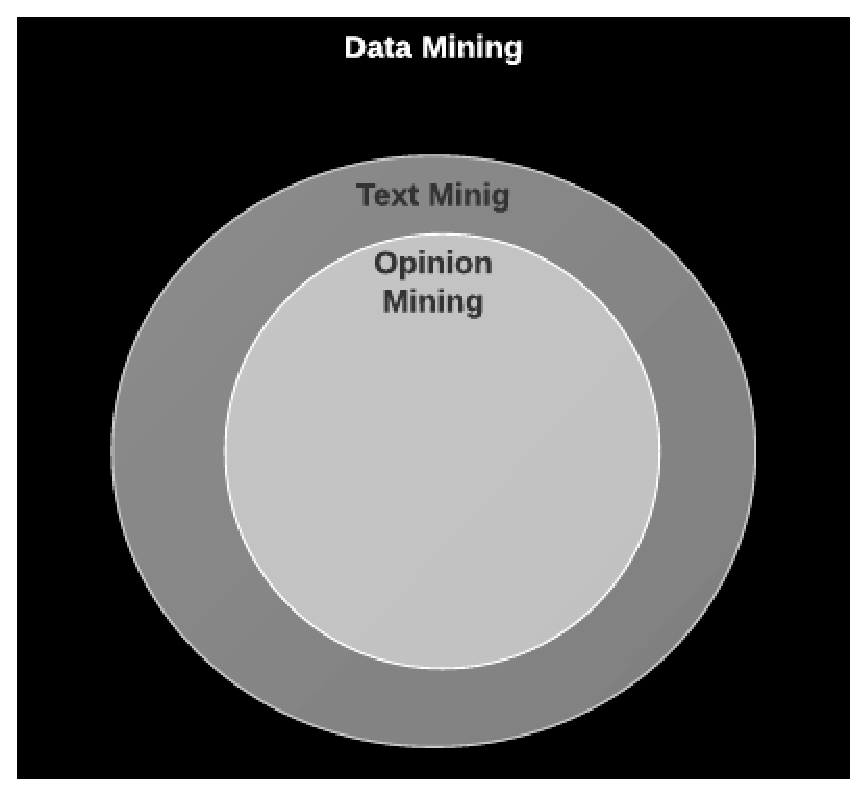
\epsfig{file=figuras/venn.eps, width=5cm}
	\caption{Diagrama de Venn - Mineração de Dados}
	\label{uni}
\end{figure}

\subsection{Sentimento}
De acordo com psicólogo Klaus R. Scherer, sentimento é um breve episódio da resposta sincronizada de todos os ou grande parte dos subsistemas orgânicos em resposta a um evento interno ou externo de grande significância\cite{scherer2001emotional}. Algumas outras definições utilizadas são:
\begin{itemize}
	\item Ato ou efeito de sentir;
	\item Aptidão para receber as impressões;
	\item Sensação, sensibilidade;
	\item Consciência íntima;
	\item Faculdade de compreender, intuição e percepção;
\end{itemize}

A mineração de opinião, também conhecida como mineração de sentimento, análise de sentimento ou extração de opinião, é um campo dentro da mineração de dados \cite{santos2014mineraccao} que tem como objetivo extrair o sentimento do texto escrito por uma pessoa, sem a interferência humana durante o processo. Porém, existe dificuldade em afirmar categoricamente o que é sentimento. 

\subsection{Desafios}

No campo de mineração de opinião, existem uma série de desafios que devem ser tidos como grandes pontos de atenção para quem deseja aplicar essa técnica de forma correta. 

\begin{itemize}
	\item Em blogs e redes sociais é comum encontrar textos com erros de ortografia ou escritos de forma informal, contendo gírias e abreviações comuns dentro da comunicação virtual;
	\item Dificuldade em discernir uma opinião ou um fato, especialmente quando existem opiniões embutidas em fatos;
	\item Os textos podem conter ironias e sarcarmos, que são especialmente difíceis de serem identificados e podem impactar os resultados;
	\item Um texto pode se referir à dois temas diferentes - política e ideologia, por exemplo - com opiniões diferentes sobre os mesmos, o que pode confundir a classificação;
\end{itemize}

\subsection{Etapas}

O processo de mineração de opinião consiste em 3 etapas: \cite{mineracaoopiniaoufsc}

\begin{itemize}
	\item Coleta de dados;
	\item Classificação;
	\item Análise dos resultados;
\end{itemize}

\subsubsection{Coleta de dados}

Nesta etapa é conduzida uma busca por opiniões nas mais diversas fontes que podem ser úteis: artigos, sites, comentários, anúncios dentre outras. Como explicado anteriormente, deve-se visar identificar se a informação coletada é uma opinião ou fato. Fatos podem ser descartados imediatamente, porém opiniões apresentadas através de fatos, podem ser úteis.

Existem diversas maneiras de coletar sistematicamente fontes para extrair e armazenar os dados que serão utilizados, dentre elas as mais famosas estão o desenvolvimento \textit{crawlers} e a utilização de APIs.

\subsubsection{Classificação}

A classificação é a alma do processo de mineração de opinião. Nesta etapa é determinada a polaridade do objeto de estudo, pretendendo determinar se o mesmo é positiva, negativa ou neutra.

Essa etapa é a principal responsável pela acurácia da análise. Por ser a etapa mais delicada do processo é onde ocorrem a maior parte dos erros. Existem diversas técnicas e ferramentas que ajudam a mitigar tais problemas que serão abordadas mais adiante, no Capítulo~\ref{cap:proposta}.

\subsubsection{Análise dos resultados}

A análise dos resultados envolve cruzar as informações de polaridade obtidas através texto com qualquer outra informação que exista sobre quem produziu aquela opinião. Desta forma, é possível, por exemplo, determinar qual gênero - masculino ou feminino - tem uma maior aceitação à um produto ou personalidade. As possibilidades para cruzar os dados e obter \textit{insights} será proporcional a quantidade de informações coletadas durante o processo.

\subsection{Aplicações práticas}

Um algoritmo capaz de extrair opiniões de um texto pode ser aplicado em diversos cenários:

\subsubsection{Pesquisa de opinião sobre um produto}

Mineração de opinião pode ser usada por uma companhia para determinar se um certo produto lançado ao mercado atingiu a aceitação prevista, como forma de entender a percepção do público e guiar estrategicamente ações de marketing e relações públicas. Ainda é possível prospectar o sentimento associado a um produto antes mesmo do seu lançamento, visando antecipar \textit{insights} que podem ser valiosos durante o seu desenvolvimento.

\subsubsection{Análise sobre pessoas públicas}

Da mesma forma, é possível utilizar a mesma técnica e direcionar as análises para uma personalidade pública. Por exemplo, é possível determinar a aceitação ou rejeição de um político durante o mandato ou período de eleições, gerando dados que podem ser decisivos na definição de suas estratégias de campanha. (REFRÊNCIA AQUI SOBRE IMPORTANCIA DE PESQUISA DE OPINIÃO NA POLÍTICA)

\subsubsection{Bolsa de valores}

Os números do mercado financeiro são uma consequência direta do sentimento que pessoas(investidores) possuem sobre uma empresa. (REFERÊNCIA SOBRE COMO MERCADO FINANCEIRO É "HUMANO" E DIRIGIDO POR EMOÇÕES) A opinião extraída de especialistas e sites de notícias podem ser usados como um dos fatores decisivos para compra e venda de ações.

\subsection{Fontes de dados}

É notório que estamos rodeados de dados dentro da Internet, porém dentro do campo de minerações de opiniões, existem algumas fontes que se destacam pela abrangência e diversidade dos dados.

\subsubsection{Mecanismos de busca}

É possível utilizar mecanismos de busca para obter opiniões sobre praticamente qualquer temática. Este método possui uma particularidade: mecanismos de busca como Google e Bing destacam certas páginas de acordo com motivos desconhecidos (RESCREVER MELHOR ISSO AQUI), o que pode influenciar os resultados obtidos. De forma geral, essa análise é apenas um reflexo do que está sendo buscado naquele momento.

Um exemplo da utilização de mecanismos de busca para mineração de opinião é o site whatdoesinternetthink.net\cite{whatdoesinternetthink}, que utiliza como base os mecanismos de busca Google e Bing para determinar a opinião sobre um tema específico ou comparar dois temas entre si.

\subsubsection{Redes sociais}

O intenso compartilhamento de informações o opiniões que vemos hoje nas redes sociais serve como uma excelente fonte de dados para a mineração de opiniões por dois motivos: diversidade e abundância. Somando-se os usuários de Facebook e Twitter por exemplo, obtemos uma amostra considerável da população mundial à disposição para pesquisas.

Para este trabalho, o Twitter foi escolhido como base para a coleta de dados, por ser uma rede social focada em opiniões de usuários e pela grande facilidade que existe em consumir os seus dados através da API pública disponibilizada pelo mesmo.

\section{Twitter}\label{sec:twitter}

Contando com uma base ativa de usuários que ultrapassa 300 milhões\cite{twittercompany2016}, o Twitter é conhecido como um \emph{microblog} fundado em março de 2006 por Jack Dorsey, Evan Williams e Biz Stone. Após 10 anos de mercado, a empresa acumula números impressionantes: 300 bilhões de mensagens já foram compartilhadas por seus usuários, que em média enviam 500 milhões de \emph{tweets}\cite{twitterstats2016} - nome pelo qual as mensagens compartilhadas no microblog ficaram conhecidas na Internet - por dia. Os usuários trocam mensagens de até 140 caracteres\cite{twittercharlimit2016} em um ambiente de rede social, que tem como objetivo dar à todos o poder de criar e compartilhar ideias e informações instantaneamente, sem barreiras\cite{twittercompany2016}. 

Dentro do Twitter, O usuário pode fazer uso de marcadores conhecidos como \emph{hashtags}\cite{waite2012paperback}, para vincular sua mensagem à um tópico específico. Apesar de simples, as \emph{hashtags} pode ser usadas das mais diversas maneiras:
\begin{itemize}
\item Agrupar comentários e pensamentos acerca de um tema
\item Estabelecer uma conexão entre dois tópicos
\item Aproximar o usuários de um conteúdo relevante com auxílio de uma busca
\end{itemize}

\subsection{Primavera Árabe}
Um dos exemplos mais recentes e impressionantes de como as redes sociais desempenharam o papel de aproximar ideologias semelhantes e encorajar debates sociais profundos foi a Primavera Árabe - onda de manifestações e protestos que tiveram início em dezembro de 2010, tendo como cenário o Norte da África e Oriente Médio. Os principais alvos foram os regimes ditatoriais e patriarcais que há muito tempo estavam no poder.\cite{howard2011opening}. Redes sociais foram amplamente utilizadas para marcar encontros, debates e manifestações, além de mostrar para o mundo o que acontecia em tempo real, através do Twitter e outras redes sociais, como o YouTube.

\begin{figure}[!h]
	\centering
\epsfig{file=figuras/primavera_arabe_redes_sociais.eps, width=10cm}
	\caption{O celular e a internet foram as armas dos rebeldes na Primavera Árabe. Fonte: Desconhecida}
	\label{uni}
\end{figure}

\subsection{Análises de redes sociais}
Este novo cenário possibilitou que a análise de redes sociais ganhasse incrível relevância nos campos de pesquisa social e comportamental\cite{wasserman1994advances}. Ao invés de analisar comportamentos individuais, atitudes e crenças, a análise de redes sociais foca sua atenção em entidades sociais ou atores interagindo entre si e como essas interações constituem uma estrutura que pode ser estudada e analisada.

Outro ponto levantado recorrentemente quando o assunto é análise de redes sociais é o como ela pode ser útil para estudos de ordem micro ou macro. No nível \textit{micro}, as análises destinam-se a examinar díades, tríades ou outros pequenos sub-grupos. No nível \textit{macro}, o objeto de estudo são grandes redes de atores sociais.
Todos os dados obtidos durante a coleta permitem segmentar os atores sociais de diversas formas - gênero, idade, religião, posição demográfica, entre outros - possibilitando análises \textit{micro} - a nível de apenas um usuário - ou \textit{macro} - quando analisamos um conjunto de usuários. Por exemplo, os dados extraídos a partir da API do Twitter, que será abordada no Capítulo 3, nos permite entender como um usuário específico reagiu a uma \textit{hashtag}. Da mesma forma, podemos olhar um cenário mais amplo, como por exemplo, todos usuários de uma região do país. As possibilidades de análise crescem e se tornam mais ricas conforme obtemos mais informações sobre os atores no momento de suas interações sociais.

\section{API}\label{sec:api}

Por definição formal, uma API é um conjunto de rotinas estabelecidos por um software para a utilização de suas funcionalidades e acessos à seus dados por outro software que não pretende entender sobre a sua implementação, apenas seus serviços. Através dessa interface, capaz de fazer uma abstração dos dados e funcionalidades de um software, conectar-se a estes serviços se torna muito mais fácil, para ambos os lados.

Outro ponto que demonstra a importância das APIs durante o desenvolvimento de software é a interoperabilidade. Atualmente, temos o mesmo serviço sendo oferecido em diferentes plataformas, como por exemplo \textit{web}, \textit{desktop}, \textit{mobile}, entre outras. Cada plataforma possui características e implementações diferentes, porém é possível que todas as plataformas utilizem as APIs como meio único de acesso a dados e serviços, promovendo uma padronização de protocolos e funcionalidades e serviços, além de alta reusabilidade de código.

\begin{figure}[!h]
	\centering\epsfig{file=figuras/interoperabilidade_api.eps, width=10cm}
	\caption{Papel das APIs integrando dados e serviços em diferentes plataformas. Fonte: http://www.programmableweb.com/}
	\label{uni}
\end{figure}

O Twitter, nossa fonte de dados durante este trabalho, possui uma API pública que pode ser utilizada por qualquer usuário da rede social \cite{twitterapidocs}. Atualmente, é a API mais utilizada no mundo, com mais de 15 bilhões de requisições por dia, 3 vezes mais acionada do que as APIs do Google, segundo colocado no ranking.

\begin{figure}[!h]
	\centering
\epsfig{file=figuras/api_mais_usada.eps, width=10cm}
	\caption{APIs mais utilizadas do mundo Fonte: SmartFile}
	\label{uni}
\end{figure}

Para efetuar uma comunicação eficiente com quem acessa à API, é necessário implementar um protocolo de acesso aos dados. Entre eles, os mais utilizados são os protocolos REST e SOAP. O primeiro é o mais popular atualmente, segundo levantamento. (REFERÊNCIA)

\subsection{REST}
O protocolo REST foi criado em 2000 por Roy Fielding \cite{fieldingrest} durante sua dissertação de doutourado na \textit{University of California Irvine}. Por ter sido criado dentro de um ambiente universitário, o objetivo do protocolo abraça a filosofia \textit{open source}. Suas principais vantagens são:

\begin{itemize}
\item Segue a filosofia \textit{open source};
\item Fácil implementação e manutenção;
\item Separa claramente a implementação do cliente e do servidor;
\item A comunicação não é controlada por uma entidade única;
\item A informação pode ser armazenada pelo cliente previnindo múltiplas chamadas;
\item Pode retornar a informação em múltiplos formatos (JSON, XML, entre outros);
\end{itemize}

Por outro lado, o protocolo REST possui algumas limitações. Entre elas, podemos destacar:

\begin{itemize}
	\item Só funciona em cima do protocolo HTTP;
	\item Autorização e recursos de segurança devem ser implementados à parte;
\end{itemize}

Baseado nessas características, o protocolo REST é comumente utilizado para APIs de aplicações \textit{Web} e \textit{Mobile}, como por exemplo, a API do Twitter, LinkedIn e Slack. (REFERÊNCIAS)

\subsection{SOAP}
Criado em 1998 por Dave Winer et al com colaboração da Microsoft (REFERÊNCIA), o protocolo SOAP foca-se em endereçar necessidades do mercado corporativo. Como vantagem, o protocolo apresenta os seguintes aspectos:

\begin{itemize}
	\item Segue uma abordagem mais formal, corporativa;
	\item Trabalha em cima de qualquer protocolo de comunicação, até mesmo assíncrono;
	\item Recursos de autorização e segurança incorporados de forma nativa;
	\item Pode ser descrito utilizando WSDL;
\end{itemize}

Entre suas principais desvantagens, podemos listar:

\begin{itemize}
	\item Gasta-se muita banda trafegando metadados
	\item Difícil e implementação
	\item Pouco popular entre desenvolvedores \textit{Web} e \textit{Mobile}
	\item Retorna informação apenas em XML
\end{itemize}

Geralmente, o protocolo SOAP é mais utilizado em serviços financeiros, \textit{gateways} de pagamento e serviços de telecomunicações.

\section{Processamento de linguagem natural}\label{sec:pnl}

\subsection{Definição}

\ac{PNL} baseia-se em modelos computacionais capazes de executar tarefas envolvem processar informações expresas em língua natural, como por exemplo, interpretação e tradução de textos. \cite{covington1994natural}.

A pesquisa na área está voltada a três aspectos da comunicação essenciais:

\begin{itemize}
	\item fonologia: estudo dos sons;
	\item morfologia: estudo da estrutura das palavras;
	\item semântica: estudo do significado;
	\item pragmática: estudo do significado aplicado a um contexto;
\end{itemize}

Neste trabalho, focaremos apenas na PNL aplicada à area da semântica e pragmática, responsável por estudar os elementos usados durante uma comunicação para se expressar através da língua (semântica) e a diversidade que pode surgir a partir de um contexto (pragmática). É também um estudo sobre como usuários de uma língua adquirem conhecimento sobre a mesma, através da comunicação oral ou escrita e como essa língua se altera ao longo do tempo.

Um dos grandes desafios da área é modelar o processamento de uma máquina para compreender uma estrutura tão complexa como uma linguagem. Existe um teste famoso na área de computação, o Teste de Turing, que levanta a questão "As máquinas podem pensar?". O artigo fundamenta conceitos chave sobre a \ac{IA}, que serve como base para o PNL.

\subsection{Teste de Turing}

Introduzido pelo matemático britânico Alan Turing em seu artigo de 1950 "\textit{Computing Machinery and Intelligence} \cite{turing1950computing}, o Teste de Turing explora a capacidade de um computador demonstrar comportamento inteligente equivalente ou indistiguível dos seres humanos.

O teste é composto por três elementos: dois seres humanos, sendo um participante e um juiz e um computador.

O juiz conversa em linguagem natural com um outro ser humano e uma máquina através de um canal de texto, composto por um teclado e uma tela que renderiza a conversa. Todos os participantes estão em ambientes separados. O juiz deve ser capaz de distinguir a máquina do ser humano, caso contrário, a máquina é considerada bem sucedida no teste. O objetivo não é analisar se a máquina é capaz de responder corretamente e sim dizer quão próximas as respostas da máquina foram das do ser humano.  

\begin{figure}[!h]
	\centering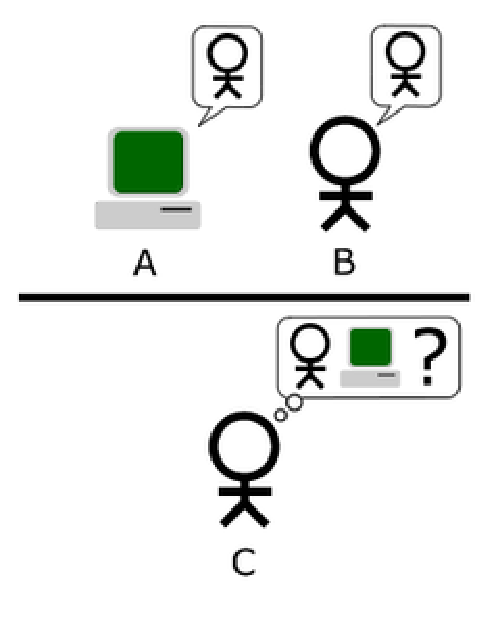
\epsfig{file=figuras/teste_turing.eps, width=10cm}
	\caption{O participante A (máquina) e o participante B (humano) se comunicam por texto com o participante C (juiz). Fonte: Wikipédia}
	\label{uni}
\end{figure}


\section{Naive Bayes (INCOMPLETO)}\label{sec:naive_bayes}
* O que é o Naive Bayes
* Demonstração matemática do algoritmo
* Uso dele em analise de sentimento/classificação


\emph{Naive Bayes} é um algoritmo probabilístico. Baseado no teorema de bayes. $$ P(A \mid B) = \frac{P(B \mid A) \, P(A)}{P(B)} $$ onde se infere qual é a probabilidade de um evento A dado um evento B. Porém nesse trabalho é utilizado o \emph{Naive Bayes} e sua diferença para o teorema de Bayes é assumir que a posição das palavras que aparecem no texto não importa, daí é acrescentado o \emph{naive}(ingênuo) ao teorema.
\\ Como visto em \cite{lucca2013implementaccao} o algoritmo computa qual a probabilidade de uma frase, denominada de documento pertencer a uma determinada classe(polaridade) \emph{P(c/d)}, a partir da probabilidade a \emph{priori} de \emph{P(c)} do documento pertencer a esta classe e da probabilidades condicionais de cada termo \emph{tk} ocorrer em um documento da mesma classe. O algoritmo tem como objetivo encontrar a melhor classe para um documento maximizando a probabilidade a\emph{posteriori} conforme a equação abaixo, onde $ n_{d} $ é o número de termos no documento \emph{d}. $$ C_{map}= argmax_{c \epsilon C}P(c|d)=argmax_{c \epsilon C}P(c)\prod 1sksn_{d}P(t_{k}/d) $$
\chapter{Proposta} \label{cap:proposta}

Como visto no Capítulo 2, existe uma corrente dentro da Mineração de Opinião que vem desenvolvendo maneiras de explorar o conteúdo digital gerado pela nossa sociedade todos os dias em redes sociais, através de técnicas utilizando Processamento de Linguagem Natural e \textit{Machine Learning}, principalmente. Com este fato surge a oportunidade de explorar novas ferramentas na
solução de problemas que envolvem pesquisas de opinião de forma geral.
Neste trabalho propõem-se um \textit{framework} que torna possível fazer pesquisas de opiniões em língua portuguesa sobre qualquer tema que seja rastreável a partir de uma \textit{hashtag} no Twitter.
Para tal é necessário que o framework criado seja capaz de:

\begin{enumerate}
	\item Coletar \textit{tweets} escritos em língua portuguesa que contenham uma determinada {hashtag};
	\item Armazenar as mensagens em uma base de dados;
	\item Classificar as mensagens de acordo com a polaridade: negativo, neutro e positivo;
	\item Extrair \textit{insights} que auxiliem a tomada de decisão a partir da massa de dados classificada;
\end{enumerate}

\section{Coleta de dados}
A plataforma do Twitter conecta aplicações e sites com seus dados através de diversos serviços. Para este trabalho, a principal fonte de dados será sua API REST, que possui uma excelente documentação disponível em \cite{twitterapidocs}. Através dela é possível acessar informações de usuários e \textit{tweets}, assim como escrever novas mensagens. Além disso, a API conta com um mecanismo de busca poderoso, que será fundamental para a coleta de dados. Os dados são entregues no formato \ac{JSON}.

\subsection{Autenticação}

Para que ter acesso à API antes é necessário possuir uma conta no Twitter e criar uma \textit{app} - através do próprio site \cite{twitterapp} - que utilizará o protocolo de autenticação OAuth\cite{oauth} para acessar os dados do Twitter se passando pelo usuário em questão. O objetivo do protocolo OAuth é permitir que uma aplicação se autentique em outra "em nome de um usuário". A aplicação pede permissão de acesso ao usuário, que possui a escolha de conceder permissão ou não. Um ponto importante: o usuário não precisa informar a sua senha para se autenticar, portanto a permissão continua vigente caso a senha do usuário se altere, o que permite que a aplicação não precise de manutenção neste caso, tornando-a mais resiliente. A autenticação por meio do OAuth necessita de três passos:

\begin{enumerate}
	\item Aplicação cliente obtém chave de autenticação;
	\item Usuário autoriza aplicação cliente na aplicação servidora;
	\item Aplicação cliente troca a chave de autenticação pela chave de acesso;
\end{enumerate}

Após o processo de criação da app, é criado um token de acesso que deve ser utilizado pelo sistema que deseja se autenticar no Twitter em nome de um usuário. Este token deve ser incorporado em cada requisição à API do Twitter para autenticar a mesma e dizer ao Twitter qual é a fonte do acesso.

\subsection{Limite de requisições}
A fim de evitar grande concentração de requisições em seus serviços, o Twitter implementa um limitador em sua API \cite{twitterrequestlimit2016}. São permitidas até 180 requisições por janela, que dura 15 minutos. Caso o limite seja ultrapassado, o serviço passa a retornar um erro na resposta, até que a "janela" de 15 minutos se renove.
A partir da versão 1.1 da API, novos cabeçalhos HTTP são retornados provendo feedback sobre os limites para requisição. Este recurso permite que o código consiga entender em que momento da janela se encontra, quantos requisições ainda podem ser feitas neste período de tempo e quanto é necessário esperar para poder fazer novas requisições. Os cabeçalhos em questão são:

\begin{itemize}
	\item X-Rate-Limit-Limit: A faixa limite para o requisição em questão;
	\item X-Rate-Limit-Remaining: O número de requisições que ainda restam para a janela de 15 minutos;
	\item X-Rate-Limit-Reset: O tempo restante dentro da janela de requisições atual, dado em segundos.
\end{itemize}

\subsection{Arquitetura}

Neste trabalho, como o objetivo é coletar \textit{tweets} postados sobre uma \textit{hashtag} em tempo real para utilizá-los como matéria-prima para análise de sentimento, é muito importante aproveitar ao máximo cada janela de requisições. Por este motivo, o sistema que coleta os dados da API do Twitter foi inspirado no modelo produtor-consumidor\cite{jeffay1993real} visando minimizar as perdas que podem acontecer em momentos de pico - como o começo ou clímax do evento, onde o volume de mensagens é maior, como veremos a frente no Capítulo 4 - e se necessário, escalar de forma simples durante os mesmos. 

\subsubsection{Produtor-consumidor}

O problema descreve dois processos, o produtor e o consumidor, que compartilham um recurso em comum usado como uma fila - um tipo particular de coleção de dados onde a primeira a entidade a entrar é a primeira a sair ou \textit{First-In-First-Out} (FIFO). A função do produtor é gerar trabalho a ser executado pelo consumidor. O volume de trabalho gerado e executado pelo sistema é controlado pela fila, que armazena as entidades ou "tarefas" a serem executadas. Essa abordagem permite que o sistema escale apenas até a sua capacidade, visto que a fila possui um tamanho fixo que caso seja ultrapassado, pode simplesmente descartar as mensagens adicionadas após este momento. Outra característica importante é a escalabilidade. Conforme os processos produtor e consumidor evoluem, surge a necessidade de aumentar a quantidade de produtores ou consumidores de forma independente.

Neste trabalho, para explorar o potencial máximo da janela de requisições foi criado um processo produtor que envia para a fila mensagens para que consumidor acesse à API do Twitter de forma que sejam feitos sempre as 180 requisições que são permitidas no intervalo de 15 minutos. Assim a responsabilidade de cada processo fica bem definida - o primeiro responde pelo volume de requisições e o segundo por realizar a requisição e entender a resposta. Para definir qual intervalo de tempo deveria ser usado para que o produtor envie mensagens à fila, foi feita uma conta simples:

$$ \frac{180}{15} = 12 \textit{ requests}_{/minuto} $$

Logo, o produtor precisa adicionar uma mensagem na fila a cada 5 segundos, para que o limite de 180 requisições seja respeitado.

\todo{Fazer diagrama do produtor-consumidor para explicar melhor}

\subsection{Busca}
Dentre os principais serviços da API do Twitter está a busca. Com ela, é possível consultar de diversas formas os principais \textit{tweets} ou mais recentes. Dentro de sua documentação, existe um guia completo de como utilizar a API  para extrair os resultados desejados \cite{twittersearchapi} das mais diversas formas. 

\subsubsection{Parâmetros adicionais}

Como abordado acima, a API possui diversos parâmetros que podem ser usados para que o usuário chegue a um conjunto de dados mais próximo da sua necessidade:

\begin{itemize}
	\item \textit{\textbf{result\_type}}: permite escolher se o resultado da busca será representado pelos \textit{tweets} mais populares (\textit{popular}) ou mais recentes (\textit{recent});
	\item \textit{\textbf{geocode}}: permite buscar por uma determinada latitude, longitude e raio, respectivamente, separando-os por vírgula. ex: geocode=-22.912214,-43.230182,1km;
	\item \textit{\textbf{lang}}: restringe os \textit{tweets} buscados a um idioma específico. ex: lang=pt;
	\item \textit{\textbf{since\_id }},  \textit{\textbf{max\_id }}, \textit{\textbf{count}} e \textit{\textbf{until}}: possibilita iterar através dos resultados quando existe um grande números de \textit{tweets} a percorrer. De acordo com a concorrência e o volume, esta tarefa pode ficar mais complicada. Uma leitura recomendada se encontra em \cite{workingwithtimelimes}.
\end{itemize}

Como o objetivo deste trabalho é coletar novos \textit{tweets} conforme eles vão sendo postados, foi necessário utilizar apenas dois parâmetros da API de busca: \textit{count} e \textit{since id}. O primeiro tem o objetivo de garantir o número máximo de registros retornados pela API e o segundo define de onde se pretende partir para buscar novos \textit{tweets}, evitando que mensagens repetidas sejam coletadas.

\url{https://api.twitter.com/1.1/search/tweets.json?q=#oscars2016&count=100&since_id=123456789}

Neste caso, a API retornará os 100 \textit{tweets} publicados desde o \textit{tweet} com identificador (\textit{id}) "123456789".

\todo{Diagrama de sequência ou atividades sobre como esta parte do código funciona}

\subsubsection{O problema com a detecção automática de idioma do Twitter}

O escopo deste trabalho determina que o objeto de estudo são apenas mensagens escritas em língua portuguesa. Como forma de obter somente \textit{tweets} escritos em língua portuguesa é preciso utilizar o parâmetro \textit{lang}, por exemplo:

\url{https://api.twitter.com/1.1/search/tweets.json?q=#oscars2016&lang=pt&result_type=recent}

Porém, realizando alguns testes na API do Twitter, foi detectado que ao submeter algum \textit{tweet}, alguma rotina dentro do próprio Twitter atribui um idioma à mensagem automaticamente. Nos testes conduzidos durante este trabalho foi identificado que em mensagens curtas - algo recorrente no Twitter - o algoritmo apresenta resultados aquém do esperado na identificação do idioma, visto que as poucas palavras contidas na mensagem podem ser comuns a mais de um idioma. Por conta disso foi decidido que o filtro de idioma não seria utilizado. Esta decisão pode mudar de acordo com o evento monitorado ou com o escopo do estudo.

\subsubsection{Escalando de forma horizontal}

Por uma questão de desenho da API de busca, cada requisição é capaz de trazer no máximo 100 \textit{tweets}, o que nos dá ao total uma carga máxima de até 1200 novos \textit{tweets} por minuto. Para as análises feitas durante este trabalho este número se mostrou mais do que suficiente. Como dito anteriormente, se fosse necessário escalar este sistema para monitorar um evento maior, seria necessário apenas obter um saldo maior de requisições junto a API do Twitter - adicionando mais tokens de usuário e criando uma espécie de "rodízio" de autenticações, por exemplo - e escalar o número de consumidores do processo de acordo com a demanda. Uma boa maneira de detectar se isso seria necessário é acompanhar quantos \textit{tweets} novos são coletados a cada requisição. Como utilizamos o \textit{id} do último \textit{tweet} capturado como referência para os novos, se a cada requisição o número de novos \textit{tweets} com grande frequência coincidir com o limite da API, temos um indício de que o volume de novas mensagens no Twitter está excedendo a capacidade do sistema de coletá-las e que o excedente está sendo perdido.

\section{Armazenamento}
A resposta da API de Busca é dada no formato JSON e cada objeto - que corresponde a cada \textit{tweet} - segue o seguinte formato e conta com diversas informações sobre o mesmo: 

\begin{lstlisting}[style=json, frame=single]
{
	"_id" : "56d388096861353c1b061fe2",
	"contributors" : null,
	"truncated" : false,
	"text" : "Leonardo DiCaprio com o #oscars eh igual a Katy Perry com o Grammy #OscarsNaTNT",
	"is_quote_status" : false,
	"in_reply_to_status_id" : null,
	"id" : 704091511902834688,
	"favorite_count" : 0,
	"source" : "<a href=\"http://twitter.com/download/android\" rel=\"nofollow\">Twitter for Android</a>",
	"created_at_datetime" : ISODate("2016-02-28T20:51:12.000Z"),
	"retweeted" : false,
	"coordinates" : null,
	"created_at_timestamp" : 1456714272.0000000000000000,
	"entities" : {
		"symbols" : [],
		"user_mentions" : [],
		"hashtags" : [{
			"indices" : [ 24, 31 ],
			"text" : "oscars"
		}, 
		{
			"indices" : [ 66, 78],
			"text" : "OscarsNaTNT"
		}],
		"urls" : []
	},
	"in_reply_to_screen_name" : null,
	"id_str" : "704091511902834688",
	"retweet_count" : 0,
	"in_reply_to_user_id" : null,
	"favorited" : false,
	"user" : {
		"follow_request_sent" : false,
		"has_extended_profile" : true,
		"profile_use_background_image" : false,
		"id" : 2786117482,
		"verified" : false,
		"profile_text_color" : "000000",
		"profile_image_url_https" : "https://pbs.twimg.com/profile_images/700450356141158404/xA-mRqp7_normal.jpg",
		"profile_sidebar_fill_color" : "000000",
		"is_translator" : false,
		"entities" : {
			"description" : {
			"urls" : []
			}
		},
		"followers_count" : 156,
		"protected" : false,
		"location" : "Um lugarzinho no fim do mundo",
		"default_profile_image" : false,
		"id_str" : "2786117482",
		"lang" : "pt",
		"utc_offset" : -28800,
		"statuses_count" : 6171,
		"description" : "Uuuumm ta estilosa!",
		"friends_count" : 192,
		"profile_background_image_url_https" : "https://abs.twimg.com/images/themes/theme1/bg.png",
		"profile_link_color" : "9266CC",
		"profile_image_url" : "http://pbs.twimg.com/profile_images/700450356141158404/xA-mRqp7_normal.jpg",
		"notifications" : false,
		"geo_enabled" : false,
		"profile_background_color" : "000000",
		"profile_banner_url" : "https://pbs.twimg.com/profile_banners/2786117482/1456444936",
		"profile_background_image_url" : "http://abs.twimg.com/images/themes/theme1/bg.png",
		"name" : "Padeira Estilosa",
		"is_translation_enabled" : false,
		"profile_background_tile" : false,
		"favourites_count" : 6095,
		"screen_name" : "naycordeir",
		"url" : null,
		"created_at" : "Fri Sep 26 18:43:47 +0000 2014",
		"contributors_enabled" : false,
		"time_zone" : "Pacific Time (US & Canada)",
		"profile_sidebar_border_color" : "000000",
		"default_profile" : false,
		"following" : false,
		"listed_count" : 1
	},
	"geo" : null,
	"in_reply_to_user_id_str" : null,
	"lang" : "pt",
	"created_at" : "Sun Feb 28 23:51:12 +0000 2016",
	"metadata" : {
		"iso_language_code" : "pt",
		"result_type" : "recent"
	},
	"in_reply_to_status_id_str" : null,
	"place" : null
}
\end{lstlisting}

Dentro desta resposta, existem diversos dados que podem ser úteis para análises em cima dos \textit{tweets} e armazená-los é extremamente valioso.

\subsection{Banco de dados orientado a documento}

Existem diversas soluções de banco de dados disponíveis no mercado. Nos últimos anos, uma delas se tornou especialmente popular\cite{bhuvan2015technical}: os bancos de dados orientado a documento. Tais bancos de dado são uma das principais categorias de bancos conhecidos NoSQL (\textit{Non Structure Query Language}) que consiste em organizar os dados de forma "não-relacional", através de documentos, gráficos, chave-valores e colunas. Bancos NoSQL são conhecidos pela facilidade de modelagem e desenvolvimento, alto desempenho de leitura e escrita, alta disponibilidade e resiliência. Isso não significa que bancos SQL são obsoletos ou piores, porém existem aplicações claras onde cada um desempenha um melhor papel. Podemos apontar algumas comparações, como por exemplo:

\begin{table}[H]
	\label{tabela-sql-nosql}
	\begin{tabular}{|m{2.5cm}|m{6cm}|m{6cm}|}
		 \hline	
		& Banco de dados relacional                                                                                                                                                                                                                            & Banco de dados NoSQL                                                                                                                                                                                                                                                                                                                \\ \hline 
		Modelagem   & O modelo relacional normaliza dados em estruturas tabulares conhecidas como tabelas, que consistem em linhas e colunas. Um schema define estritamente as tabelas, colunas, índices, relações entre tabelas e outros elementos do banco de dados.     & Bancos de dados não relacionais (NoSQL) normalmente não aplicam um schema. Geralmente, uma chave de partição é usada para recuperar valores, conjuntos de colunas ou documentos semiestruturados JSON, XML ou outros que contenham atributos de itens relacionados.                                                                  \\ \hline 
		Desempenho  & O desempenho normalmente depende do subsistema do disco. A otimização de consultas, índices e estrutura de tabela é necessária para alcançar máximo desempenho.                                                                                      & Desempenho geralmente é uma função do tamanho do cluster do hardware subjacente, da latência de rede e da aplicação que faz a chamada.  \\ \hline 
		Escala      & Mais fácil de aumentar a escala "verticalmente" com hardware mais rápido.,Outros investimentos são necessários para tabelas relacionais para abranger um sistema distribuído.                                                                        & Projetado para aumentar a escala "horizontalmente" usando clusters distribuídos de hardware de baixo custo para aumentar a transferência sem aumentar a latência.                                \\ \hline 
		APIs & As solicitações para armazenar e recuperar dados são comunicadas usando consultas compatíveis com structured query language (SQL). Essas consultas são analisadas e executadas por sistemas de gerenciamento de bancos de dados relacionais (RDBMS). & APIs baseadas em objetos permitem que desenvolvedores de aplicações armazenem e restaurem facilmente estruturas de dados na memória. As chaves de partição permitem que os aplicativos procurem pares de chave-valor, conjuntos de colunas ou documentos semiestruturados contendo objetos e atributos de aplicativos serializados. \\ \hline 
	\end{tabular}
		\caption{Comparação entre bancos SQL e NoSQL}
\end{table}

\subsection{Opções disponíveis}
O movimento de adoção de bancos \textit{NoSQL} está bastante enraizada no mundo \textit{open source}. Alguns projetos como Voldemort\cite{voldemortproject}, MongoDB\cite{mongodb}, Tokyo Cabinet\cite{tokyocabinet} e CouchDB\cite{couchdb}. Apesar de uma grande quantidade de opções \textit{open source}, o movimento ganhou muita força com a publicação de duas publicações sobre implementações proprietárias: o Google BigTable\cite{chang2008bigtable} e o Amazon Dynamo\cite{decandia2007dynamo}. Para este trabalho, a opção escolhida foi o MongoDB, altamente popular na comunidade \textit{open source} e com bastante material disponível com melhores práticas de criação, manutenção e configuração.

\subsection{Armazenando \textit{tweets}}
O objetivo deste trabalho é monitorar eventos através das \textit{hashtags}. E para cada uma delas é criada uma coleção - nome dado a um conjunto de documentos - dentro do banco de dados. O nome da coleção é dado pela \textit{hashtag} monitorada.

No momento onde o processo consumidor - responsável por fazer requisições na API e lidar com o retorno - é ligado ocorre a criação da coleção, caso a mesma não exista, e dentro dela começam a ser armazenados os \textit{tweets} retornados pela API, obedecendo ao mesmo formato enviado pelo Twitter. A flexibilidade dAntes do armazenamento no banco alguns campos a mais são adicionados, mas vamos entrar neste detalhe apenas na seção sobre Classificação.

\section{Classificação}
\begin{itemize}
	\item Aplicar técnicas de normalização no texto. As mesmas devem ser específicas para a língua portuguesa;
	\item Construir base de palavras e termos classificados utilizadas como insumo para o modelo matemático;
	\item Preparar uma massa de treino para validar o modelo matemático antes da execução;
	\item Calibragem do algoritmo
	\item Salvar infos sobre a classificação dentro do documento
\end{itemize}

\subsection{Normalização do texto}

A composição de um \textit{tweet} escrito por muitas vezes possui elementos que serão inúteis ou nocivos para o nosso algoritmo de classificação. Por conta disso, um dos primeiros desafios para tal é conduzir uma normalização nas mensagens, que serão nosso objeto de estudo.


\subsection{Construção da base de palavras e termos}
A construção da base de dados foi feita com o intuito de melhor expressar um sentimento de uma palavra ou texto, para a utilização do algoritmo. Para isso a base foi dividida em dois arquivos, positivos e negativos. Além dessa divisão foi utilizada outas bases criadas como: Re-li(referencia), SentiLex-PT \cite{marioj.silvapaulacarvalholuissarmento2012}, base da puc \cite{freitas2013construccao}, emoticons \cite{alexanderhogenboomdaniellabalflaviusfrasincarmalissabalfranciskadejonguzaykaymak}. Todas usando a língua portuguesa ou um linguajar universal, no caso dos emoticons e já estarem polarizadas. Essas bases têm em comum é serem feitas apenas de palavras, então ficou-se a dúvida de como a classificação funcionaria posteriormente quando aplicadas a um texto que as palavras podem não estar no mesmo contexto. Ex: "O flamengo jogou muito mal, mas fico feliz pela vitória", onde tem a palavra mal que já dá um tom negativo a frase , porém ao terminar de ler a frase encontrasse as palavras feliz e vitória que tem um contexto positivo.
Com essas bases já citadas foi compreendida a necessidade de uma base mais específica para o linguajar utilizado na internet, constituído de  
gírias, abreviação e até erros de português, para isso foi criada uma base utilizando dados pegos do twitter a partir da marcação hashtagoscar2016.


\subsection{Massa de treino}

\subsection{Massa de teste}

\subsection{Algoritmo}



\chapter{Resultados e análises}\label{cap:resultados}

Nesta seção será apresentada os resultados obtidos e os processos necessários para a obtenção dos mesmos. Como visto no Capitulo 4 uma das fases necessárias para a Análise de Sentimento é a classificação de polaridade dos \textit{tweets}. Durante a classificação, que era o resultado da execução do Naive Bayes, foram utilizadas diversas formas de execução que serão apresentadas abaixo

\section{Cenários e parâmetros de teste}\label{sec:cenarios}
Durante a execução dos testes para a análise de resultados o ambiente utilizado foi:
\begin{itemize}
	\item Sistema operacional: Linux Ubuntu
	\item Processador: Core i7
	\item Memória: 8GB
	\item Quantidade de \textit{tweets}: 141798
\end{itemize}


\section{Experimentos realizados e resultados}\label{sec:resultados}
O primeiro teste realizado para a classificação da base obteve o seguinte resultado:
\todo{Trazer tabela  1 pra ca}
\begin{table}[]
	\caption{1º teste}
	\label{teste-1}
	\resizebox{\textwidth}{!}{%
		\begin{tabular}{|l|l|r}
			\hline
			\multicolumn{3}{|c|}{1º Teste} \\ \hline
			\multicolumn{2}{|l|}{Bases usadas} & \multicolumn{1}{r|}{Tecnicas usadas} \\ \hline
			\multicolumn{2}{|c|}{Sentilex} & \multicolumn{1}{c|}{Stopwords} \\
			\multicolumn{2}{|c|}{PUC} & \multicolumn{1}{c|}{Stemming} \\ \cline{3-3} 
			\multicolumn{2}{|c|}{ReLi} &  \\ \hline
			\multicolumn{3}{|c|}{Resultado} \\ \hline
			\multicolumn{2}{|l|}{Positivo} & \multicolumn{1}{r|}{17350} \\ \hline
			\multicolumn{2}{|l|}{Negativo} & \multicolumn{1}{r|}{15517} \\ \hline
			\multicolumn{2}{|l|}{Neutro} & \multicolumn{1}{r|}{108931} \\ \hline
			\multicolumn{2}{|l|}{Tempo} & \multicolumn{1}{r|}{311.673 segundos} \\ \hline
		\end{tabular}%
	}
\end{table}

Analisando a tabela \ref{teste-1} é visto quais as bases utilizadas, nesse caso, Reli , PUC e Sentilex, as técnicas utilizadas nesse teste, \textit{Stopwords} e \textit{Stemming}, e o resultado que de 141798 \textit{tweets}, 17350 foram positivos, 15517 negativos e 108931 neutros, levando 311.673 segundos para executar o teste.
\todo{Adicionar imagem}

Observando os resultados, é visto que a quantidade de \textit{tweets} neutros é maior que a dos outros, com isso foi que havia a necessidade de diminuir a quantidade de neutros. Mudanças no cenário de testes para conseguir essa diminuição. 
\todo{Tabela 2 aqui}

\begin{table}[]
	\caption{2º teste}
	\label{teste-2}
	\resizebox{\textwidth}{!}{%
		\begin{tabular}{|l|l|r}
			\hline
			\multicolumn{3}{|c|}{2º Teste} \\ \hline
			\multicolumn{2}{|l|}{Bases usadas} & \multicolumn{1}{r|}{Tecnicas usadas} \\ \hline
			\multicolumn{2}{|c|}{Sentilex-Stem} & \multicolumn{1}{c|}{Stopwords-Stem} \\
			\multicolumn{2}{|c|}{PUC-Stem} & \multicolumn{1}{c|}{Stemming} \\ \cline{3-3} 
			\multicolumn{2}{|c|}{ReLi} &  \\ \hline
			\multicolumn{3}{|c|}{Resultado} \\ \hline
			\multicolumn{2}{|l|}{Positivo} & \multicolumn{1}{r|}{49263} \\ \hline
			\multicolumn{2}{|l|}{Negativo} & \multicolumn{1}{r|}{35079} \\ \hline
			\multicolumn{2}{|l|}{Neutro} & \multicolumn{1}{r|}{57456} \\ \hline
			\multicolumn{2}{|l|}{Tempo} & \multicolumn{1}{r|}{397.48 segundos} \\ \hline
		\end{tabular}%
	}
\end{table}

No 2º teste visto na tabela \ref{teste-2} é visto que a quantidade de neutro diminuiu consideravelmente, apenas aplicando a técnica de \textit{stemming} nas bases de palavras
\todo{grafico 2}


Ainda buscando a diminuição de neutros foi criada uma base de palavras mas próxima do domínio que esse trabalho propõe que é o Oscar2016, essa base contem palavras relevantes a esse evento, gerando o seguinte resultado.
\todo{colocar tabela 3 aqui}

\begin{table}[]
	\caption{3º teste}
	\label{teste-3}
	\resizebox{\textwidth}{!}{%
		\begin{tabular}{|l|l|r|}
			\hline
			\multicolumn{3}{|c|}{3º Teste} \\ \hline
			\multicolumn{2}{|l|}{Bases usadas} & Técnicas usadas \\ \hline
			\multicolumn{2}{|c|}{Oscar2016} & \multicolumn{1}{c|}{\textit{Stopwords}} \\ \hline
			\multicolumn{3}{|c|}{Resultado} \\ \hline
			\multicolumn{2}{|l|}{Positivo} & 47450 \\ \hline
			\multicolumn{2}{|l|}{Negativo} & 7210 \\ \hline
			\multicolumn{2}{|l|}{Neutro} & 87138 \\ \hline
			\multicolumn{2}{|l|}{Tempo} & 709,126 segundos \\ \hline
		\end{tabular}%
	}
\end{table}

Analisando a tabela \ref{teste-3} é visto que apenas uma base mais especializada no domínio não consegue diminuir a quantidade de neutros e ainda aumenta o tempo para a execução dos testes.
\todo{grafico 3}


No 4º teste foi adicionada o base criada, Oscar2016, com as bases genéricas, gerando o seguinte resultado:
\begin{table}[]
	\caption{4º teste}
	\label{teste-4}
	\resizebox{\textwidth}{!}{%
		\begin{tabular}{|c|l|r}
			\hline
			\multicolumn{3}{|c|}{4º Teste} \\ \hline
			\multicolumn{2}{|l|}{Bases usadas} & \multicolumn{1}{r|}{Técnicas usadas} \\ \hline
			\multicolumn{2}{|c|}{Oscar2016} & \multicolumn{1}{c|}{Stopwords} \\
			\multicolumn{2}{|c|}{SentiLex} & \multicolumn{1}{c|}{Stemming} \\ \cline{3-3} 
			\multicolumn{2}{|c|}{PUC} & \multicolumn{1}{c}{} \\
			\multicolumn{2}{|c|}{ReLi} & \multicolumn{1}{c}{} \\ \hline
			\multicolumn{3}{|c|}{Resultado} \\ \hline
			\multicolumn{2}{|l|}{Positivo} & \multicolumn{1}{r|}{69070} \\ \hline
			\multicolumn{2}{|l|}{Negativo} & \multicolumn{1}{r|}{33461} \\ \hline
			\multicolumn{2}{|l|}{Neutro} & \multicolumn{1}{r|}{39267} \\ \hline
			\multicolumn{2}{|l|}{Tempo} & \multicolumn{1}{r|}{650.97 segundos} \\ \hline
		\end{tabular}%
	}
\end{table}

Analisando a tabela \ref{teste-4} é visto que nesse teste foi obtida a maior diminuição de neutros, mas com um tempo de processamento um pouco maior.
\todo{Adicionar grafico 4}

Segue abaixo um comparativo dos testes.

\begin{table}[]
	\caption{Comparando testes}
	\label{teste-comp}
	\resizebox{\textwidth}{!}{%
		\begin{tabular}{l|l|c|l|l|}
			\cline{2-5}
			\multicolumn{1}{c|}{} & \multicolumn{1}{c|}{Teste 1} & Teste 2 & \multicolumn{1}{c|}{Teste 3} & \multicolumn{1}{c|}{Teste 4} \\ \hline
			\multicolumn{1}{|l|}{Positivo} & 15517 & \multicolumn{1}{r|}{49263} & 47450 & 69070 \\ \hline
			\multicolumn{1}{|l|}{Negativo} & 17350 & 35079 & 7210 & 33461 \\ \hline
			\multicolumn{1}{|l|}{Neutro} & 108931 & \multicolumn{1}{l|}{57456} & 87138 & 39267 \\ \hline
			\multicolumn{1}{|l|}{Tempo (s)} & \multicolumn{1}{c|}{311.673} & 397.48 & 709.129 & 650.97 \\ \hline
		\end{tabular}%
	}
\end{table}

\chapter{Conclusão} \label{cap:conclusao}

Este trabalho identificou e abordou a importância que a mineração de opinião possui nos dias atuais, além das oportunidades que este novo campo de estudo abre com a sua descoberta: tanto na área acadêmica quanto para exploração comercial e estratégica e assim como propôs, desenvolveu uma solução capaz de extrair mensagens escritas em língua portuguesa de uma \textit{hashtag} do Twitter e classificá-las em positivas, neutras ou negativas, tornando possível fazer análises de mineração de opinião que são capazes de interpretar como um universo de usuários se sente em relação a temática estudada. Sem dúvida, o grande desafio foi mostrar que é viável aplicar uma solução de mineração de opinião mesmo com a complexidade da língua portuguesa.
Com base no que foi apresentado, a proposta cumpriu os seguintes objetivos levantados:

\begin{itemize}
	\item Utilização do Twitter como plataforma de dados;
	\item Construção um processo escalável capaz de extrair mensagens de uma \textit{hashtag} do Twitter;
	\item Utilização bases de palavras classificadas disponíveis na literatura sobre o tema;
	\item Aplicação de técnicas de normalização de texto visando um maior desempenho ao classificar;
	\item Implementação do algoritmo de \textit{Naive Bayes} para classificar as mensagens em positivas, neutras ou negativas;
	\item Conduzir a classificação em mensagens que foram escritas em língua portuguesa;
	\item Aplicação do conhecimento adquirido durante este trabalho em um estudo de caso utilizando a cerimônia do Oscars 2016;
	\item Demonstração dos cenários de teste e seus impactos no resultado final;
	\item Análise dos resultados obtidos atraves de gráficos que permitem interpretar os sentimentos dos usuários antes, durante e depois do evento, sob diversas perspectivas.
\end{itemize}

A análise dos resultados mostrou que por existir uma ansiedade muito grande vinculada aos instantes que antecedem o evento existe uma grande concentração de sentimentos positivos atrelados a este momento. Outro fato que ficou evidente é que os momentos mais populares do evento, como o anúncio das categorias mais aguardadas como: melhor ator, melhor atriz e melhor filme são as mais esperadas e com a confirmação da vitória dos favoritos, houve um pico de mensagens positivas por volta do horário do anúncio dos vencedores destas categorias. Outros dois momentos chamaram atenção pela carga de sentimentos negativos: o show de David Grohl em homenagem aos falecidos no mundo do cinema em 2015 onde a sensação de luto ficou evidente e a apresentação de Lady Gaga, onde o tema do filme que a música  faz parte da trilha sonora aborda estupros em faculdades americanas, tema que desperta bastante tristeza nas pessoas que sofreram este tipo de trauma ou que empatizam de alguma forma com as vítimas deste crime.


\section{Trabalhos Futuros}\label{sec:8_trabfut}

Como visto neste trabalho, o algoritmo utilizado para gerar os resultados das classificações a fim de realizar a análise de sentimento foi o \textit{Naive Bayes}. Para trabalhos futuros pode-se utilizar outros algoritmos como: Árvore de Decisão, Regressão Logística, \textit{Maximum Entropy Model}. Podendo ser usados somente o próprio algoritmo ou realizando um trabalho comparativo entre eles, descobrindo qual algoritmo gera melhores resultados.

Outro método que pode ser utilizado é a aplicação de \textit{n-grams}, para averiguar o melhor desempenho do modelo. Com isso poderia-se realizar testes de acurácia, que não foi o enfoque deste trabalho. Pode-se também utilizar outras fontes de dados, não só o Twitter, como: Facebook, fórums, comentários de sites, entre outros. Mais um fator relevante são as bases, que nesse trabalho foram utilizadas três bases genéricas e uma pequena base personalizada, então como trabalho futuro propõem-se utilizar apenas bases personalizadas e referentes ao domínio.

Durante as pesquisas para esse trabalho foi encontrado um \textit{toolkit}  para a técnica de \textit{word embedding}, conhecido como \textit{word2vec}, criado em 2013 por uma equipe do Google. Esse tipo de técnica se baseia em redes neurais, que difere do algoritmo probabilístico utilizado nesse trabalho. Sendo essa uma outra proposta pra trabalhos futuros.

Entre os testes realizados no capítulo \ref{cap:resultados} foi presenciado um fator instigante. A duração dos testes,  que podem ser encontrados no apêndice \ref{teste_tempo},  foi notado um crescimento anômalo, entretanto não foi discutido a causa de tal crescimento, então é proposto um estudo onde se discute tal anomalia. 

Por fim, pretende-se fazer o máximo para desenvolver o  processamento de linguagem natural para a língua portuguesa, onde técnicas e métodos serão comparadas visando o melhor desempenho com uma análise mais profunda e a automação da inteligência artificial para o aproveitamento desse campo para o ser humano em suas tomadas de decisão. 



% --- -----------------------------------------------------------------
% --- Referencias Bibliograficas. (Obrigatorio)
% --- -----------------------------------------------------------------
\cleardoublepage
%\bibliographystyle{acm-2} 
%\bibliographystyle{abnt-num} % abbrv - abnt-num
\inputencoding{latin1}
\bibliographystyle{IEEEtran}
%\bibliographystyle{uff-ic}
\bibliography{referencia} % arquivo fonte com a bibliografia
%\bibliography{articles,books,standards,websites} % arquivo fonte com a bibliografia

\cleardoublepage

\renewcommand{\appendixtocname}{Ap\^{e}ndice}
\chapter{Bases de texto utilizadas}

\section{\textit{PUC}}
\subsection{Termos negativos}
anticl\'{i}max besteira bobagem bo\c{c}al bosta chatice clich\^{e} decep\c{c}\~ao defeito demorar desastre desconforto desesperan\c{c}a desgra\c{c}a desprazer droga engano erro exagero exaust\~ao excesso falhar falho falta furo imaturidade inc\^{o}modo inexperiente lixar meleca melodrama melodram\'{a}tico meloso mundo nojo passividade pena pieguice porca porcaria problema sacrif\'{i}cio sentimentalismo superficialidade vergonha abandonar aborrecer arrepender assustar aterrorizar atormentar atrapalhar cansar chocar complicar decepcionar deprimir desanimar desgastar desistir desmerecer destorcer detestar dificultar distorcer empacar enfraquecer enganar engolir errar estragar estressar exagerar faltar frustrar incomodar irritar largar limitar odiar pecar perder prolongar revoltar aborrecente \'{a}gua-com-a\c{c}\'{u}car anacr\^{o}nico besta bestar bizarro bobo burro cansativo chato chocante chulo clich\^{e} confuso construir decepcionante defeituoso deplor\'{a}vel depressivo deprimente desagrad\'{a}vel desconexo desgastante desinteressante desnecess\'{a}rio desprez\'{i}vel dif\'{i}cil dispens\'{a}vel doentio ego\'{i}sta enfadonho enjoado enjoativo entediante esdr\'{u}xulo estereotipado estranho falsar falso fraco frio frustrante f\'{u}til gra\c{c}a horr\'{i}vel horroroza idiota idiotice imaturo impaciente impressionar incompreens\'{i}vel inconsistente ing\^{e}nuo injustific\'{a}vel insuport\'{a}vel intermin\'{a}vel in\'{u}til irritante lament\'{a}vel ma\c{c}ante machista mal manjado massa mau mediano m\'{e}dio meloso mero modinha morno negativo normal obsessivo oco opressivo pat\'{e}tico pesaroso p\'{e}ssimo piegas piorar plana pobre pomposo pregui\c{c}oso previs\'{i}vel puritano rasa raso razo\'{a}vel reacion\'{a}rio reclamo repa repetitivo repulsivo revoltante rid\'{i}culo ruim sem simplista sofr\'{i}vel superficial surreal t\'{e}dio tedioso tenda tongo tosco triste vazio violento vol\'{u}vel est\'{a}tico id\^{e}ntico lento linear 

\subsection{Termos positivos}
alegria ast\'{u}cia atemporalidade beleza bem-estar best-seller brilho carisma cl\'{i}max companheirismo compreens\~ao deleite densidade diferencial divers\~ao do\c{c}ura emo\c{c}\~ao empatia entusiasmo envolvente \^{e}xtase f\~a facilidade fascina\c{c}\~ao favorito flu\^{e}ncia fluidez genialidade gostinho grandeza intelig\^{e}ncia ironia magnetismo m\'{e}rito obra-prima originalidade paix\~ao perfei\c{c}\~ao prazer predileto preferido primor sensibilidade sufocamento talento taquicardia ternura top virtude adorar agradar amadurecer amar animar apaixonar apegar apreciar aprender arrebatar arrebentar atrair cativar conquistar curtir deliciar destacar-se divertir emocionar emplacar empolgar encantar enternecer entreter facilitar fascinar fluir gostar identificar inovar recomendar sensibilizar simpatizar valorizar vibrar viciar apavorar brilhar comover devorarprender rir saborearsurpreender tocar admir\'{a}vel ador\'{a}vel agrad\'{a}vel alegre alucinante apaixonante ardente arrasador arrebatador astuto atemporal aterrador atraente atual atuar aut\^{e}ntico avassalador bacana b\'{a}rbaro batuta bel\'{i}ssimo belo bem bem-humorado bom bonito brilhante carinhoso carism\'{a}tico cativante cativar certo claro classe cl\'{a}ssico coerente com\'{e}dia c\^{o}mico comovente compreens\'{i}vel comum consistente contagiante contente convincente corajoso criativo crivar curto decente delicado delicioso demais denso desafiador despretensioso devanear digno direto distrativo divertido divino doce duro elegante eletrizante emocionante empolgante encantador encant\'{a}vel engenhoso engra\c{c}ado enigm\'{a}tico enriquecedor envolvente especial esperto espetacular espirituoso espl\^{e}ndido essa estonteante excelente excepcional excitante exemplar extraordin\'{a}rio fabuloso face f\'{a}cil fama fant\'{a}stico fascinante fascinate favorito feliz fluente fluido foder fofo forte fren\'{e}tico fundamental genial gostoso gotoso grande grandioso gratificante grato hil\'{a}rio humano ideal imcompar impactante impag\'{a}vel impar \'{i}mpar impec\'{a}vel imperd\'{i}vel importante impressionante inabal\'{a}vel inacredit\'{a}vel incr\'{i}vel indescrit\'{i}vel indispens\'{a}vel in\'{e}dito inesquec\'{i}vel infal\'{i}vel inovador inquietante inquieto inspirador instigante instingar inteligente intenso interessante \'{i}ntimo intrigante irado ir\^{o}nico irresist\'{i}vel jovial legal leg\'{i}timo leve li\c{c}a light linda lindo l\'{i}rico m\'{a}gico magistral magn\'{e}tico magnificar magn\'{i}fico majestoso maravilha maravilhoso marcante massa m\'{a}ximo mel\'{i}fluo memor\'{a}vel minucioso misterioso moderno not\'{a}vel novo obra ode original palp\'{a}vel pass\'{a}vel perfeito pertinente plaus\'{i}vel poderoso po\'{e}tico pontual positivo precioso predileto primo primoroso prof\'{e}tico profundo pungente r\'{a}pido raro razo\'{a}vel real realista real\'{i}stico recente recomendar recomend\'{a}vel reflexivo relaxante relevante rico sagaz seco sedutor seguro sensacional sens\'{i}vel sensual sentimental s\'{e}rio sexy significativo simples sincero singelo singular sublime subversivo surpreso surreal teres tocante tranquilo transl\'{u}cido \'{u}ltimo v\'{a}lido verdadeiro veross\'{i}mil vertiginoso viciante vicioso vigoroso visceral vital voraz arrasador aterrorizante assustador angustiante compulsivo fren\'{e}tico imprevis\'{i}vel surpreendente sufocante perturbador sombrio

\section{\textit{ReLi}}
\subsection{Termos negativos}
\'{a}gua com a\c{c}\'{u}car \'{a}gua-com-a\c{c}\'{u}car cabe\c{c}a-dura carregar nas tintas dar n\'{a}useas dar raiva dar sono deixar a desejar embrulhar o est\^{o}mago esperar mais for\c{c}ar a barra mala sem al\c{c}a melhor esquecer n\~ao aturar n\~ao engolir n\~ao prestar nao se enxergar perder o f\^{o}lego picol\'{e} de chuchu pra criancinha quebrar o encanto sem gra\c{c}a sem sal sem-no\c{c}\~ao ser um balde de \'{a}gua fria ser um saco tempo perdido perder tempo perda de tempo aborrecente anacr\^{o}nico besta bizarro bobo burro cansativo chato chocante chulo clich\^{e} confuso decepcionante defeituoso deplor\'{a}vel depressivo deprimente desagrad\'{a}vel desconexo desgastante desinteressante desnecess\'{a}rio desprez\'{i}vel dif\'{i}cil dispens\'{a}vel doentio ego\'{i}sta enfadonho enjoado enjoativo entediante esdr\'{u}xulo estereotipado estranho falso fraco frio frustrante f\'{u}til horr\'{i}vel horroroza idiota idiotice imaturo impaciente incompreens\'{i}vel inconsistente ing\^{e}nuo injustific\'{a}vel insuport\'{a}vel intermin\'{a}vel in\'{u}til irritante lament\'{a}vel ma\c{c}ante machista mal manjado mau mediano m\'{e}dio meloso mero modinha morno negativo normal obsessivo oco opressivo pesaroso p\'{e}ssimo piegas piorar plana pobre pomposo pregui\c{c}oso previs\'{i}vel puritano raso razo\'{a}vel reacion\'{a}rio repetitivo repulsivo revoltante rid\'{i}culo ruim simplista sofr\'{i}vel superficial surreal t\'{e}dio tedioso tenda tongo tosco triste vazio violento vol\'{u}vel est\'{a}tico id\^{e}ntico lento linear anticl\'{i}max besteira bobagem bo\c{c}al bosta chatice clich\^{e} decep\c{c}\~ao defeito demorar desastre desconforto desesperan\c{c}a desgra\c{c}a desprazer droga engano erro exagero exaust\~ao excesso falhar falho falta furo imaturidade inc\^{o}modo inexperiente lixar meleca melodrama melodram\'{a}tico meloso mundo nojo passividade pena pieguice porca porcaria problema sacrif\'{i}cio sentimentalismo superficialidade vergonha abandonar aborrecer arrepender assustar aterrorizar atormentar atrapalhar cansar chocar complicar decepcionar deprimir desanimar desgastar desistir desmerecer destorcer detestar dificultar distorcer empacar enfraquecer enganar engolir errar estragar estressar exagerar faltar frustrar incomodar irritar largar limitar odiar pecar perder prolongar revoltar


\subsection{Termos positivos}
abrir a mente abrir a minha mente amor \`{a} primeira vista arrancar l\'{a}grimas arrancar risadas arrancar gargalhadas capturar a aten\c{c}\~ao chamar a aten\c{c}\~ao com chave de ouro dar certo de corpo e alma de encher os olhos de fazer inveja de tirar o f\^{o}lego deixar de boca aberta estar louco para faltar adjetivos faltar palavras fazer pensar fora de s\'{e}rie gostinho de quero mais grata surpresa ir a nocaute lindo de morrer morrer de rir n\~ao ter adjetivos para pra ningu\'{e}m botar defeito ser show ser um show ser um achado ser um tapa na cara soco na boca de o est\^{o}mago ter f\^{o}lego tudo de bom valer cada N valer a pena admir\'{a}vel ador\'{a}vel agrad\'{a}vel alegre alucinante apaixonante ardente arrasador arrebatador astuto atemporal aterrador atraente atual atuar aut\^{e}ntico avassalador bacana b\'{a}rbaro batuta bel\'{i}ssimo belo bem bem-humorado bom bonito brilhante carinhoso carism\'{a}tico cativante cativar certo claro classe cl\'{a}ssico coerente com\'{e}dia c\^{o}mico comovente compreens\'{i}vel comum consistente contagiante contente convincente corajoso criativo crivar curto decente delicado delicioso demais denso desafiador despretensioso devanear digno direto distrativo divertido divino doce duro elegante eletrizante emocionante empolgante encantador encant\'{a}vel engenhoso engra\c{c}ado enigm\'{a}tico enriquecedor envolvente especial esperto espetacular espirituoso espl\^{e}ndido essa estonteante excelente excepcional excitante exemplar extraordin\'{a}rio fabuloso face f\'{a}cil fama fant\'{a}stico fascinante fascinate favorito feliz fluente fluido foda fofo forte fren\'{e}tico fundamental genial gostoso gotoso grande grandioso gratificante grato hil\'{a}rio humano ideal imcompar impactante impag\'{a}vel impar \'{i}mpar impec\'{a}vel imperd\'{i}vel importante impressionante inabal\'{a}vel inacredit\'{a}vel incr\'{i}vel indescrit\'{i}vel indispens\'{a}vel in\'{e}dito inesquec\'{i}vel infal\'{i}vel inovador inquietante inquieto inspirador instigante instingar inteligente intenso interessante \'{i}ntimo intrigante irado ir\^{o}nico irresist\'{i}vel jovial legal leg\'{i}timo leve li\c{c}a light linda lindo l\'{i}rico m\'{a}gico magistral magn\'{e}tico magnificar magn\'{i}fico majestoso maravilha maravilhoso marcante massa m\'{a}ximo mel\'{i}fluo memor\'{a}vel minucioso misterioso moderno not\'{a}vel novo obra ode original palp\'{a}vel pass\'{a}vel perfeito pertinente plaus\'{i}vel poderoso po\'{e}tico pontual positivo precioso predileto primo primoroso prof\'{e}tico profundo pungente r\'{a}pido raro razo\'{a}vel real realista real\'{i}stico recente recomend\'{a}vel reflexivo relaxante relevante rico sagaz seco sedutor seguro sensacional sens\'{i}vel sensual sentimental s\'{e}rio sexy significativo simples sincero singelo singular sublime subversivo surpreso surreal teres tocante tranquilo transl\'{u}cido \'{u}ltimo v\'{a}lido verdadeiro veross\'{i}mil vertiginoso viciante vicioso vigoroso visceral vital voraz arrasador aterrorizante assustador angustiante compulsivo fren\'{e}tico imprevis\'{i}vel; surpreendente sufocante perturbador sombrio alegria ast\'{u}cia atemporalidade beleza bem-estar best-seller brilho carisma cl\'{i}max companheirismo compreens\~ao deleite densidade diferencial divers\~ao do\c{c}ura emo\c{c}\~ao empatia entusiasmo envolvente \^{e}xtase f\~a facilidade fascina\c{c}\~ao favorito flu\^{e}ncia fluidez genialidade gostinho grandeza intelig\^{e}ncia ironia magnetismo m\'{e}rito obra-prima originalidade paix\~ao perfei\c{c}\~ao prazer predileto preferido primor sensibilidade sufocamento talento taquicardia ternura top virtude adorar agradar amadurecer amar animar apaixonar apegar apreciar aprender arrebatar arrebentar atrair cativar conquistar curtir deliciar destacar-se divertir emocionar emplacar empolgar encantar enternecer entreter facilitar fascinar fluir gostar identificar impressionar inovar recomendar sensibilizar simpatizar valorizar vibrar viciar apavorar brilhar comover devorar prender rir saborear surpreender tocar

\section{\textit{SentiLex}}
\subsection{Termos negativos}
abafado abafante abaixado abalado abalroado abandalhado abandalhamento abandonado abandonar abarrotado abatido abelhudo aberra\c{c}\~ao aberrante aberrativo abespinhado abestalhado abilolado abje\c{c}\~ao abjec\c{c}\~ao abjecto abjeto abobado abobalhado abolido abominador abominando abomin\'{a}vel aborrecer-se aborrecido abortado abrupto abrutalhado absentista abstracto abstra\'{i}do abstrato abstrusidade abstruso absurdo abulia ab\'{u}lico abusado abusador abusar abusivo acabado acabadote acabrunhado acaciano a\c{c}ambarcador acanhado acanhamento acanhar-se ac\'{e}falo acerado acerbidade acerbo ac\'{e}rrimo achacado achatado achincalhar acidentado aciganado acintoso acirrado acobardado acobardar-se acobertado acocado a\c{c}oitado acomodadi\c{c}o acomodar-se acordar com o rabo para o ar acordar com os p\'{e}s de fora acorrentado acorrentar-se acossado a\c{c}ougueiro acre acrian\c{c}ado acr\'{i}tico aculturado acusado acutilante adiposo admoestador adoentado adormecido adulador adulterador adulterino adult\'{e}rio ad\'{u}ltero adverso a\'{e}reo afanado afasia af\'{a}sico afectado afeminado afetado afiado afli\c{c}\~ao afligido afligir-se aflitivo aflito afobado afogado afogar as m\'{a}goas afogar-se em pouca \'{a}gua afogar-se afrontado afrontoso afundado afundan\c{c}o afundar-se agachado agarotado agarrado agarrar-se ao poder agastadi\c{c}o agastado agastar-se agiota agir de m\'{a}-f\'{e} agoirento agonia agoniado agoniante agoniar agonizante agoureiro agourento agravado agravar agre agredir agressividade agressivo agressor agreste agrilhoado agrosseirado aguado agu\c{c}ado alapado alarmante alarmismo alarmista alarve alarvice albino alcoolismo alcoolizado alegado aleijado aleivoso algemado alheado alhear-se alheio aliciado aliciar aliena\c{c}\~ao mental alienado alien\'{i}gena alquebrado altaneiro altivo aluado alucina\c{c}\~ao alucinado alucinar alumbrado alvora\c{c}ado amachucado amadorismo amaldi\c{c}oado amalucado amaneirado amarelado amarelo amargado amargo amargura amargurado amaricado amarrado amassado ambiguidade amb\'{i}guo ambiopia ambliopia amea\c{c}a amea\c{c}ador amea\c{c}ante amedrontado amedrontador amigo da on\c{c}a amigo da pinga amigo dos copos amn\'{e}sia amn\'{e}sico amolecer amoral amoralidade amoralista amorfia amorfo amortecido amotinado amputado amuado amuamento amuar amuo anafado analfabeto an\~ao an\'{a}rquico anarquista andante andar a apanhar bon\'{e}s andar \`{a} deriva andar a dormir \`{a} sombra da bananeira andar a dormir andar a falar sozinho andar \`{a} nora andar a pensar na morte da bezerra andar a reboque de andar \`{a} sombra da bananeira andar ao deus dar\'{a} andar aos bon\'{e}s andar aos ca\'{i}dos andar aos pap\'{e}is andar armado em carapau de corrida andar \`{a}s aranhas andar \`{a}s cavalitas de andar \`{a}s cegas andar \`{a}s turras com andar com a cabe\c{c}a na lua andar com cara de caso andar com dor de corno andar com dor de cotovelo andar com macacos na cabe\c{c}a andar com macaquinhos na cabe\c{c}a andar com o cora\c{c}\~ao nas m\~aos andar com os azeites andar de olhos vendados andar de trombas andar em pele e osso andar feito barata tonta andar feito com andar na boa vida andar na lua andar na m\'{a} vida andar pelos cabelos andrajoso an\'{e}mico an\^{e}mico anestesiado angustiado angustiante animal animosidade aniquilado anjinho anor\'{e}ctico anor\'{e}tico anorexia nervosa anorexia anormal anormalidade anotia ansioso anti-republicano antidemocrata antidesportista antidesportivismo antiliberal antiliberalista antinatural antipatia antip\'{a}tico antipatriota antipatriotismo antipol\'{i}tico antiquado antisocial apagado apagar-se apalermado apalha\c{c}ado apancado apanhado apanhar nas orelhas apanhar por tabela apaparicar aparolado apartado aparvalhado apatetado apatia ap\'{a}tico apatriota apavorado apavorante apavorar-se apeado apedantado apedrejado apedrejar aperaltado aperreado aplicar golpes baixos a apopl\'{e}ctico apopl\'{e}tico apoquentado apoquentador apreendido apreensivo apriorista aprisionado aprontar apropriar-se aproveitador aproveitar-se apunhalado apunhalar pelas costas apunhalar aquietador arbitr\'{a}rio arcaico ardil ardiloso \'{a}rduo arfante \'{a}rido arisco armar barraca armar-se aos c\'{a}gados armar-se aos cucos armar-se em carapau de corrida armar-se em chico esperto armar-se em parvo armar-se arquejante arranhado arranjar lenha para se queimar arranjar sarna para se co\c{c}ar arranjar um bico de obra arrasado arrastadeiro arrastado arrebentado arrebitado arredado arredio arreliado arreliador arrenegado arrepender-se arrepiante arrepio arrevesado arrivista arrogante arrolado arruaceiro arrufado arrufo arruinado arruinamento arruinar-se arruinar arrumar as botas arteirice arteiro arteriosclerose artificial artificialidade artif\'{i}cio artificiosidade artificioso artimanha artritismo aselha aselhice asfixiante asilado asneira asneirento asno aspereza \'{a}spero asquerosidade asqueroso assalariado assaloiado assaltante assaltar assanhadi\c{c}o assanhado assarapantado assassinar assassino assediado assediador assediar ass\'{e}dio sexual ass\'{e}dio assim\'{e}trico assoberbado assolado assolador assomadi\c{c}o assombrado assustadi\c{c}o assustado assustador assustar-se astenia ast\'{e}nico ast\'{u}cia astucioso astuto atabalhoa\c{c}\~ao atabalhoado atabalhoamento atacante atado atafulhado atamancado ataranta\c{c}\~ao atarantado atarantar-se atarracado ateado atemorizado aterrado aterrador aterrorizado aterrorizador atirar areia para os olhos de atirar barro \`{a} parede atirar com as culpas a atirar poeira aos olhos de atoleimado at\^{o}nito atordoado atordoador atormentado atormentador atracado atrai\c{c}oado atrapalhado atrapalhar-se atrasado mental atrasado atraso mental atraso atravessadi\c{c}o atravessado atribulado atroador atrocidade atrofia atrofiado atrofiante atrofiar-se atrofiar atropelado atropelar atroz atulhado aturdido austero autismo autista autodestrui\c{c}\~ao autodestrutivo autorit\'{a}rio autoritarismo avarento avareza avariado avariar avaro avassalador avassalamento avassalante averso avesso \'{a}vido aviltado aviltador aviltante avinagrado avinhado avulso azafamado azambrado azar azarado azarento azedar azedo azedume azeiteiro azelha azelhice azoinante azougado babaca bab\~ao baboseira babosice baboso ba\c{c}o para espelho bacoco bacoquice badalhoco badalhoquice bagaceiro bagunceiro baixeza baixote bajulador bajular balbuciante balofice balofo bambo banal banalidade banalizar banana bancarrota bandido banditismo banido banzado baralhado baralhar-se barato barbaridade b\'{a}rbaro barrado barraqueiro barrigana barrigudo barroco barulhento baselga b\'{a}sico bastardo batatudo bater a bota bater as botas bater com o nariz na porta bater no ceguinho bater no fundo batido batota batoteiro batotice beatice beato b\^{e}bado bebedeira b\^{e}bedo bebedor beberr\~ao bebido bebum bei\c{c}udo belfo belicismo belicista b\'{e}lico belicoso bem mandado bera besta bestificado bexiguento bibliomania bilioso biltre bimbo biqueiro bira birra birrento biruta bisbilhotar bisbilhoteiro bisbilhotice bisonho bizarria bizarro blasfemador blasf\'{e}mia blasfemo bloqueado bloquear boateiro bobo boboca bo\c{c}al bocejar bochechudo bo\^{e}mio bo\'{e}mio bojudo bolachudo bolorento bombeado borbulhento borguista borrachudo borrado boto botocudo bravateador brega brejeirice brejeiro brejeirote briga brigador brigante brig\~ao briguento brilharete brincar bronco bronquice bruno brusco brutal brutalidade brutid\~ao bruto bruxaria bucha bufismo bufo bulh\~ao bulhento bul\'{i}cio buli\c{c}oso burgu\^{e}s burla burlado burlador burl\~ao burlesco burlista burrice burro cabazada cabe\c{c}a dura cabe\c{c}udo cabisbaixo caboclo cabotino cabr\~ao c\'{a}bula ca\c{c}ado cacete caceteiro cachaceiro cadastrado cadav\'{e}rico cadaveroso cadente caduco cafona cag\~ao cagar-se cagarola cagativo caguinchas ca\'{i}do caipira cair na armadilha cair na boca do lobo cair na ratoeira cair por terra cair calaceiro cal\~ao calar a boca calar o bico calar-se calcado calculismo calculista calhandreiro calhandrice calhorda calino caloteirismo caloteiro calotismo cal\'{u}nia caluniado caluniador caluniar cambada cambaleante cambalear camelo canalha canalhice canceroso cancro candongueiro candonguice cangalheiro canhestro canibal canino cansado cansativo cantar bem mas n\~ao me alegra cantar de galo capcioso capenga capitoso capricho caprichoso caqu\'{e}ctico caqu\'{e}tico caquexia cara de cu cara de pau caralho carapa\c{c}a carbonizado carcomido carecer carecido careiro car\^{e}ncia carenciado carente caricato carnavalesco carniceiro carrancudo casmurrice casmurro casquilho cassete castigado castigador castra\c{c}\~ao castrador catalepsia catano cataplexia catarro catatonia catinguento cativo caturra caturrice causador caustica\c{c}\~ao causticante causticidade c\'{a}ustico cavern\'{i}cola cavernoso caviloso ceder cego cegueira cegueta celerado censurado cepo cercado chalaceiro chalado chamuscado chanfrado chantagista charlatanice charlat\~ao chateado chatice chato chauvinismo chauvinista chav\~ao cheio de nove horas cheirar a mofo chibante chicaneiro chico esperto chicoteador chifrudo chinesada chinesice chinfrim chinfrim chinfrineiro chocalheiro chocar chocarreiro chochice chocho choco chon\'{e} choraming\~ao choramingar choramingas chor\~ao chorar sobre o leite derramado chorar choroso chulo chumbado chumbar chunga chupado chupador chupismo chupista cigano cilindrado cil\'{i}ndrico c\'{i}nico cioso cisma cismado cism\'{a}tico ci\'{u}me ciumento clamoroso clandestino claudicante claustrofobia cleptomania cleptoman\'{i}aco coagido coagir coartado cobarde cobardia cobardola cobi\c{c}a cobi\c{c}oso cocainomania coercivo cogitabundo cogita\c{c}\~ao cogitativo coio coitado colaboracionista colapso col\'{e}rico comandita combalido combalimento com\'{e}dia comedor comer gato por lebre comer o p\~ao que o diabo amassou comichento comichoso comil\~ao comodismo comodista compactuar comparsa compelido compelir complexado complicado comprado comprar gato por lebre comprometedor compulsivo compungido comuna conceituoso condenado conden\'{a}vel condescend\^{e}ncia condo\'{i}do condoreiro conflituosidade conflituoso conformado conformar-se conformista confrangedor confranger-se confundido confundir alhos com bugalhos confundir-se confus\~ao confuso congelado congest\~ao congestionado conivente conluiado conspira\c{c}\~ao conspirador conspirativo conspurcar consterna\c{c}\~ao consternado consternador consternar constipado constrangedor constranger constrangido constrangimento consumido consumir-se consumista contagiado contagioso contaminar contendedor contendente contentar-se com pouco contestado contido contingente contorcer-se contracto contradizer-se contra\'{i}do contrair-se contranaturo contrariado contrista\c{c}\~ao contristado contrito controlador controv\'{e}rsia controverso controvertido contumaz contund\^{e}ncia contundente contundido contuso convulsivo coquete corcovado corcunda cornudo cornuto correr a toque de caixa corrido corriqueiro corroer-se corroer corromper corrompido corrosivo corrup\c{c}\~ao corrupt\'{i}vel corruptivo corrupto corruptor cortado cortar na casaca de coscuvilheiro covarde covardia coveiro coxo cr\'{a}pula crapuloso crasso cretinice cretinismo cretino criancice criminalidade criminoso crispa\c{c}\~ao crispado crispar-se critic\'{a}vel crivado cromo cru crucificador cruel crueldade crueza cruzar os bra\c{c}os culpa culpado culpas culposo curto de vistas curvado curvar-se curvil\'{i}neo curvo cuspido danado danificado danoso dar \`{a} l\'{i}ngua dar \`{a} sola dar \`{a} soleta dar a volta ao miolo dar ao p\'{e} dar bandeira dar barraca dar cabo da vida a dar com a boca no trombone dar com a l\'{i}ngua nos dentes dar com os burros na \'{a}gua dar com os p\'{e}s a dar de frosques dar graxa a dar o corpo ao manifesto dar o dito por n\~ao dito dar o golpe a dar o golpe do ba\'{u} dar palmadinhas nas costas a dar pontap\'{e}s na gram\'{a}tica dar tiros nos p\'{e}s dar um pontap\'{e} no cu a dar um tiro no p\'{e} dar uma no cravo e outra na ferradura dar voltas no caix\~ao deambula\c{c}\~ao deambulante deambular debandado d\'{e}bil debilidade debilita\c{c}\~ao debilitado debochado deboche decad\^{e}ncia decadente decadentista deca\'{i}do decepado decep\c{c}\~ao decepcionado decepcionante decepcionar decrepidez decr\'{e}pito defeituoso defensiva defesso deficiente definhado definhamento deforma\c{c}\~ao deformado defraudar as expectativas de defraudar defunto degenerado degradado degradante degredado degredo deicida deitar achas na fogueira deitar as unhas a deitar foguetes antes da festa deitar lenha na fogueira deitar poeira aos olhos a deitar poeira para os olhos de deitar tudo a perder deitar tudo para tr\'{a}s das costas deitar tudo por \'{a}gua abaixo deixar com as cal\c{c}as na m\~ao deixar com as m\~aos a abanar deixar de rastos deixar muito a desejar deixar o barco \`{a} deriva deixar o pa\'{i}s de tanga deixar tudo para depois deixar-se levar delambido delet\'{e}rio delinqu\^{e}ncia delinquente delirar delituoso demagogia demagogo demarcado dem\^{e}ncia demente dem\'{e}rito demitido d\'{e}mod\'{e} demolidor demon\'{i}aco demorado denegrido denegrir a sua imagem dengoso depauperado depenado dependurado deplora\c{c}\~ao deplor\'{a}vel deportado deposto deprava\c{c}\~ao depravado depravador depreciado depreciar depreciativo depress\~ao man\'{i}aca depress\~ao depressivo depressor deprim\^{e}ncia deprimente deprimido derramado derreado derreamento derrota derrotado derrotismo derrotista derrubado desabonado desabrido desabrigado desabusado desacompanhado desacordado desacreditado desactualizado desadaptado desafecto desafeto desafina\c{c}\~ao desafinado desaforado desaforido desafortunado desagradado desagrad\'{a}vel desagradecido desagrado desaire desairoso desajeitado desajustado desalentado desalento desalinhado desalinhamento desalmado desalojado desamparado desamparo desanima\c{c}\~ao desanimado desanimador desapaixonado desaparafusado desaparecer do mapa desaparecido desapegado desapiedado desapontado desapontador desapossado desapropriado desaprovador desaproveitado desarranjado desarrazoado desarrumado desarticulado desassisado desassossegado desassossego desastrado desastre desastroso desatento desatinado desatualizado desaustinado desavergonhado desavisado desbaratado desbaratador desbocado desbocamento desbotado desbragado descabelado descabelar-se descabido descadeirado descalabro descal\c{c}o descamisado descarado descaramento descarnado descascado descautelado descer ao mais baixo n\'{i}vel descer nas sondagens descerrado desclassificado descomedido descomedimento desconcentra\c{c}\~ao desconcentrado desconcertado desconexo desconfiado desconfort\'{a}vel desconhecedor desconsidera\c{c}\~ao desconsola\c{c}\~ao desconsolado descontentamento descontente descontrolado descontrolo descoordena\c{c}\~ao descoordenado descorado descoro\c{c}oado descort\^{e}s descortesia descuidado descuido desd\'{e}m desdenhar desdenhoso desdentado desdito desditoso deselegante desemparelhado desempregado desemprego desencalhe desencaminhado desencaminhador desencaminhamento desencontrado desengon\c{c}ado desengra\c{c}ado desenxabidez desenxabido desequilibrado desequil\'{i}brio desertar desertor desesperado desesperan\c{c}a desesperan\c{c}ado desespero desestabilizador desfalcar desfalecido desfasado desfavorecido desfeito desfigurado desgarrado desgastado desgaste desgosto desgostoso desgoverna\c{c}\~ao desgovernado desgoverno desgra\c{c}a desgra\c{c}ado desgracioso desgrenhado desidrata\c{c}\~ao desiludido desinfeliz desinforma\c{c}\~ao desinformado desinstru\'{i}do desinteressado desinteressante desinteresse desistir deslambido deslavado desleal deslealdade desleixado desleixar-se desleixo desligado deslocado desmaiado desmanchado desmantelado desmazelado desmazelamento desmazelo desmedido desmemoriado desmentido desmesurado desmiolado desmontado desmoraliza\c{c}\~ao desmoralizado desmoralizador desmoronar-se desmotiva\c{c}\~ao desmotivado desmotivador desnaturado desnorteado desnorteamento desnutri\c{c}\~ao desobedi\^{e}ncia desobediente desocupado desola\c{c}\~ao desolado desolador desolhado desonestidade desonesto desonra desonrado desonrar desonroso desordeiro desordem desordenado desorganiza\c{c}\~ao desorganizado desorienta\c{c}\~ao desorientado despassarado despeitado despeitar despeito despeitorado despejado despenteado despercebido desperdi\c{c}ado desperdi\c{c}ador despesista despirocado despistado desplante despregado despreocupa\c{c}\~ao despreven\c{c}\~ao desprevenido desprezado desprez\'{a}vel desprez\'{i}vel desprezo desprimoroso desproporcionado despropositado desprotegido despudor despudorado desqualificado desregrado desregulado desremediado desrespeitado desrespeitador desrespeitar desrespeito desrespeitoso destabilizador destampado destapado destemperado desterrado destoante destrambelhado destrambelhamento destratado destravado destro\c{c}ado destro\c{c}o destrui\c{c}\~ao destru\'{i}do destruidor destrutivo destrutor desumanidade desumano desunido desusado desvairado desvairamento desvalido desvanecer desvantagem desvariado desvario desventurado desventuroso desviar dinheiro desvirtuado desvitalizado deteriorado deteriorar detestado detest\'{a}vel detido detrator deturpado deturpar devaneador devassado devassid\~ao devasso devastado devastador dever comer farinha maizena dever dobrar a l\'{i}ngua dever ter vergonha na cara devoto de Baco diabolismo difama\c{c}\~ao difamado difamador difamar dif\'{i}cil difuso digressionista digressivo dilacerado diminu\'{i}do d\'{i}scolo discrimina\c{c}\~ao discriminado discriminador discriminar disfar\c{c}ado disfonia disforme disformidade dislexia disl\'{e}xico disparatado disparatar disparate dispens\'{a}vel dispersivo disperso displic\^{e}ncia displicente dissidente dissimula\c{c}\~ao dissimulado dissimular dissipado dissipador dissoluto dissolvido distante distorcer distorcido distra\'{i}do ditador divaga\c{c}\~ao divagador divagante divagar dizer cobras e lagartos de dizimado doente doentio dogm\'{a}tico dogmatista doidivanas doido de todo doido varrido doido dolente dolorido doloso dominado dopado dopagem dorido dorm\^{e}ncia dormente dorminhoco dormitar doudo draconiano dram\'{a}tico dramatismo dramatizar dr\'{a}stico droga drogado dromomania dromoman\'{i}aco dubiedade d\'{u}bio dubitativo duficuldades d\'{u}plice duplicidade duro da mioleira duro de ouvido duro duvidoso edipiano efeminado ego\'{i}smo ego\'{i}sta egotista eleg\'{i}aco elei\c{c}oeiro elitista emaciado emaranhado emba\c{c}ado embaciado embara\c{c}ado embara\c{c}o embara\c{c}oso embasbacado embatucado embirra\c{c}\~ao embirrante embirrento embotado embriagado embrulhado embruxado embu\c{c}ado embuchado emburrado embuste embusteiro emp\'{a}fio empalidecido empalmado empanturrado empapu\c{c}ado empedernido empedernimento emperrado emperramento empertigado empobrecido empoeirado empolado emporcalhado emproado emulador \^{e}mulo encabulado encalacra\c{c}\~ao encalacrado encalhado encalhamento encamado encanado encarcerado encarni\c{c}ado encavacado enciumado enclausurado encoberto encobrir encolerizado encolerizar-se encolher os ombros encolhido encostar-se a encovado encruado encurralado encurralamento encurvado endemoniado endemoninhado endiabrado endividado endividamento endividar-se endividar endoidecer endurecido enerva\c{c}\~ao enervado enervamento enervante enervar-se enfadado enfadamento enfadar-se enfadonho enfardador enfartado enfartamento enfastiado enfastiamento enfastiante enfatuado enfeiti\c{c}ado enfermi\c{c}o enfermidade enfezado enfezamento enfiado enfiar o barrete enforcar-se enfraquecer enfraquecido enfrascado enfronhado enfunado enfurecer-se enfurecido enfurecimento engaiolado engaiolamento enganado enganador enganar-se enganar engano enganoso engarrafado engasgado engasgamento engatado engodado engolfado engolido engolir em seco engonha engrupido enigm\'{a}tico enjeitado enjoado enjoar enjoo enlameado enleado enlevado enlouquecer enlouquecido enlouquecimento enlutado enojado enojar enraivecido enraivecimento enrascada enrascado enredado enregelado enresinado enrijecido enrodilhador enrolado enrugado ensacado ensanguentado ensanguentado ensimesmado ensimesmamento ensurdecedor entalado entalar-se entaramelado entediado entediante enterrado enterrar a cabe\c{c}a na areia enterrar-se entontecido entontecimento entornado entorpecer entorpecido entorpecimento entortado entregador entregar a alma ao criador entregar a alma ao diabo entregar o ouro ao bandido entreva\c{c}\~ao entrevado entristecer entristecido entristecimento entubado entulhado entumecimento envaidecido envelhecido envenenador envenenamento envenenar envergonhado envergonhar-se envergonhar enviesado envinagrado enxerido enxofrado enxoframento enxovalhado epigram\'{a}tico epil\'{e}tico equivocado equivocar-se equ\'{i}voco equ\'{i}voco ermo erotomania erotoman\'{i}aco errado errante errar err\'{a}tico erro esbaforido esbanjado esbanjador esbanjamento esbanjar dinheiro esbatido esborratado esburacado escabelado escabrosidade escabroso escaldado escamado escamoso escamotear escancarado escandalizar escandaloso escangalhado escanifrado escanzelado escapadi\c{c}o escapo escarnecedor escarnecido escarninho esc\'{a}rnio escarrapachado escavacado escaveirado esclerosado esclerose esconder a verdade esconder-se esconder escondido esconso escoriado escorra\c{c}ado escorregadio escorregar escrachado escravizado esculachado escuro escusado escuso esdr\'{u}xulo esfaimado esfalfado esfarrapado esf\'{e}rico esf\'{i}ngico esfomeado esgalgado esgana\c{c}\~ao esganado esgani\c{c}ado esgazeado esgazeamento esgotado esgotamento esgotante esgrouviado esguedelhado esmagado esmilhafrado esmorecer esmorecido esmorecimento espalhafato espalhafatoso espalhan\c{c}o espampanante espancado esparramado espatifado espaventoso espavorido especado espertalh\~ao espetaculoso espetado espetar-se ao comprido espezinhado espinhento espinhoso espremido esp\'{u}rio esqu\'{a}lido esquecedi\c{c}o esquecido esquel\'{e}tico esquentado esquinado esquisitice esquisito esquivo esquizofrenia esquizofr\'{e}nico esquizoidia estabanado estacado estafado estagnado estagnar estalado estalar o verniz estampado estancado estanhado estapaf\'{u}rdio estar a anos luz de estar \`{a} beira do precip\'{i}cio estar \`{a} deriva estar a dormir \`{a} sombra da bananeira estar a dormir estar a falar para as paredes estar a falar sozinho estar a jeito estar \`{a} nora estar a pensar na morte da bezerra estar \`{a} rasca estar \`{a} rasquinha estar a secar estar \`{a} sombra da bananeira estar ao deus dar\'{a} estar armado em carapau de corrida estar \`{a}s aranhas estar \`{a}s cegas estar \`{a}s turras com estar com a cabe\c{c}a na lua estar com a corda ao pesco\c{c}o estar com a corda na garganta estar com a corda no pesco\c{c}o estar com a l\'{a}grima no canto do olho estar com cara de caso estar com dor de corno estar com dor de cotovelo estar com macacos na cabe\c{c}a estar com macaquinhos na cabe\c{c}a estar com o cora\c{c}\~ao nas m\~aos estar com os azeites estar com os p\'{e}s para a cova estar com um aperto no cora\c{c}\~ao estar de cabe\c{c}a quente estar de m\~aos a abanar estar de m\~aos atadas estar de m\~aos e p\'{e}s atados estar de molho estar de olhos vendados estar de p\'{e}s atados estar de tanga estar de trombas estar em baixo de forma estar em baixo estar em peda\c{c}os estar em pele e osso estar enterrado at\'{e} \`{a}s orelhas estar feito ao bife estar feito barata tonta estar feito com estar fora de si estar na lua estar na retranca estar nas m\~aos de estar num beco sem sa\'{i}da estar pelos cabelos estar por um fio estar sempre a bater na mesma tecla estar-se nas tintas estarola estarolice estarrecido estatelado estatelar-se est\'{a}tico estavanado estendido estereotipado est\'{e}ril esterilidade esticado esticar o pernil estigmatizado estiloso estirado estoirado estoiro estourado estouvado estr\'{a}bico estragado estrangeirado estrangulado estranho estratagema estremunhado estridente estroina estropiado estruturado estulto estupefaciente estupidez est\'{u}pido estuporado estuprado esvair-se em sangue esvaziado etilizado eunuco evas\~ao evasivo evitar exacerbado exagerado exagerar exalado exaltado exaltar-se exangue exaspera\c{c}\~ao exasperado exasperar-se exasperar exaust\~ao exausto exceder-se excessividade excessivo exclu\'{i}do excomungado execra\c{c}\~ao execrado execr\'{a}vel executado exibicionismo exibicionista exibido exibir-se exilado eximido exot\'{e}rico expatriado expelido experimentar dificuldades explorador explorar explosivo expropriado expulso extenua\c{c}\~ao extenuado extenuante extravagante extraviado extremista fa\c{c}anhudo faccioso fac\'{i}nora facinoroso fadiga fadigado fal\'{a}cia falacioso falar de barriga cheia falar demais falar para as paredes falar para o boneco falar sem convic\c{c}\~ao fal\^{e}ncia falhado falhan\c{c}o falhar falho falibilidade falido fal\'{i}vel falsear falseta falsidade falso faltar \`{a} palavra faltar ao compromisso faltar ao respeito falto faltoso fam\'{e}lico faminto fanfarr\~ao fanho fanhoso fantasiar fantasista fareleiro farisaico fariseu farrista farronqueiro farsa farsante farsista farsola fascista fastidioso fastio fatal fatalista fatigado fatigante f\'{a}tuo favorecer fazer \`{a} custa de fazer a folha a fazer asneira fazer beicinho fazer biquinho fazer caretas fazer fa\'{i}sca fazer figura de urso fazer figura triste fazer filmes fazer gato e sapato de fazer horas fazer m\'{a} figura fazer orelhas moucas fazer ouvidos de mercador fazer uma rica parelha fazer uma tempestade num copo de \'{a}gua fazer vista grossa fazer-se de v\'{i}tima febril fechado fechar os olhos fechar-se em copas fedor fedorento feio feiticista feiti\c{c}o felino femeeiro ferido ferino fero feroz ferrado ferrenho f\'{e}rreo ferver em pouca \'{a}gua fescenino fetichista ficar a apanhar bon\'{e}s ficar a chupar no dedo ficar \`{a} deriva ficar a dormir \`{a} sombra da bananeira ficar a falar para as paredes ficar a falar sozinho ficar a jeito ficar \`{a} nora ficar a pensar na morte da bezerra ficar a secar ficar \`{a} sombra da bananeira ficar \`{a} sombra de ficar a ver navios ficar ao deus dar\'{a} ficar aos ca\'{i}dos ficar \`{a}s aranhas ficar \`{a}s cegas ficar com a cabe\c{c}a em \'{a}gua ficar com a cabe\c{c}a na lua ficar com as cal\c{c}as na m\~ao ficar com cara de caso ficar com dor de corno ficar com dor de cotovelo ficar com macacos na cabe\c{c}a ficar com macaquinhos na cabe\c{c}a ficar com o cora\c{c}\~ao nas m\~aos ficar com os louros ficar de m\~aos a abanar ficar de m\~aos atadas ficar de m\~aos e p\'{e}s atados ficar de molho ficar de p\'{e}s atados ficar de tanga ficar de trombas ficar em peda\c{c}os ficar em \'{u}ltimo ficar enterrado at\'{e} \`{a}s orelhas ficar feito barata tonta ficar fora de si ficar mal visto ficar na lua ficar nas m\~aos de ficar num beco sem sa\'{i}da ficar para tio ficar pelos cabelos ficar reduzido a nada ficar reduzido a zero ficar sem argumentos fict\'{i}cio filho da puta finado fincado fingido fingidor fingimento fingir fisgado fiteiro fitinhas fi\'{u}za flagelado flagelante flatul\^{e}ncia flatulento fl\'{e}bil fodido fofoqueiro fofoquice foleirice foleiro folgado fome foragido forasteiro for\c{c}ado fornicador forreta fosco fracalhote fracassado fracassar fracasso fraco fracote fr\'{a}gil fragilidade fragilizado fragmentado franzino fraqueza fraturado fraude fraudulento fren\'{e}tico frieza frigidez fr\'{i}gido frio frito frivolidade fr\'{i}volo frouxid\~ao frouxo fruste frustra\c{c}\~ao frustrado frustrar fugidio fugido fugir \`{a} quest\~ao fugir \`{a} responsabilidade fugir a sete p\'{e}s fugir ao fisco fugir \`{a}s perguntas fugir \`{a}s responsabilidades fugir com o rabo \`{a} seringa fugir fugitivo fuj\~ao fulminante fulo fundamentalista funesto furibundo furioso furtar furtivo f\'{u}til futilidade gabar-se gabarola gabiru gadelhudo gafo gag\'{a} gago gaguez gaiteiro gald\'{e}rio gamar gan\^{a}ncia gandulagem gandulo gangrena ganir ganzado garganeiro garotice garoto gaseado gastador gastar mundos e fundos gasto gatuno gaud\'{e}rio gelado g\'{e}lido genioso gentinha gentio ging\~ao glut\~ao goliardo golpeado gorado gordanchudo gordo gorducho gordurento gorduroso gozador gozo grafomania grafoman\'{i}aco grazina gringo gritante grosseir\~ao grosseirismo grosseiro grosseria grosso grotesco grudento guerra guloso handicap hediondez hediondo hemiplegia herege heresia her\'{e}tico herm\'{e}tico herodiano heroinomania hesitante heterog\'{e}neo heterog\^{e}neo hiperactivo hiperativo hiperconservador hiperconservadorismo hipercr\'{i}tico hipersensibilidade hipersens\'{i}vel hipnotiza\c{c}\~ao hipnotizado hipnotizar hipnotiz\'{a}vel hipocondria hipocondr\'{i}aco hipocrisia hirsuto histeria hist\'{e}rico homicida homic\'{i}dio homiziado horrendo horribilidade horr\'{i}fico horripila\c{c}\~ao horripilante horr\'{i}vel horror horrorizar horroroso hostil hostilidade humilhado humilhar-se idiota idiotia idiotice ignaro ignom\'{i}nia ignominioso ignorado ignorante ignoto ilegal ileg\'{i}timo ileg\'{i}vel iletrado iliberal iliteracia iliterato il\'{o}gico ilogismo iludido iludir ilus\~ao ilus\'{o}rio imaturidade imaturo imbecil imbecilidade imerecido imisericordioso imitador imitar imitativo imobilizado imodera\c{c}\~ao imoderado imod\'{e}stia imodesto imoral imoralidade imorigerado im\'{o}vel impaciente impante impatriota impecunioso impelido impenetr\'{a}vel impenitente impercept\'{i}vel impercet\'{i}vel imperdo\'{a}vel imperfei\c{c}\~ao imperfeito imperial imperialista imperiosidade imperioso imperito imperman\^{e}ncia impermanente imperscrut\'{a}vel impertin\^{e}ncia impertinente impessoal impessoalidade impetuosidade impetuoso impiedade impiedoso \'{i}mpio implac\'{a}vel implicado implicante implicativo implorar impondera\c{c}\~ao imponderado impontual impontualidade impopular impopularidade importunado importuno imposs\'{i}vel imposto impostor impostura impot\^{e}ncia impotente imprecis\~ao impreciso impregnado impreparado impression\'{a}vel imprestabilidade imprest\'{a}vel imprevid\^{e}ncia imprevidente improced\^{e}ncia improcedente improducente improdutividade improdutivo imprud\^{e}ncia imprudente impudente impudic\'{i}cia impudico impugnado impulsivo impuro imputado imund\'{i}cie imundo in\'{a}bil inabilidade inabord\'{a}vel inaceit\'{a}vel inacess\'{i}vel inactividade inactivo inadaptado inadequado inadmiss\'{i}vel inamov\'{i}vel inanima\c{c}\~ao inanimado in\^{a}nime inaplicado inapresent\'{a}vel inapto inatividade inativo inautenticidade inaut\^{e}ntico incapacidade incapaz incaracter\'{i}stico incauto incendiado incendi\'{a}rio incensador incerteza incerto inchado incipiente incivil incivilidade incivilizado inclem\^{e}ncia inclemente incoer\^{e}ncia incoerente inc\'{o}gnito incomodado incomodativo incomodidade inc\^{o}modo inc\'{o}modo incompet\^{e}ncia incompetente incompleto incompreensibilidade incompreens\'{i}vel inconceb\'{i}vel inconcili\'{a}vel inconcluso inconfess\'{a}vel inconfidente incongru\^{e}ncia incongruente inconsci\^{e}ncia inconsciente inconsequente inconsequente inconsiderado inconsist\^{e}ncia inconsistente inconsolado inconsol\'{a}vel inconstante incontin\^{e}ncia incontinente incontrari\'{a}vel incontrolado inconveni\^{e}ncia inconveniente inconvers\'{a}vel incorre\c{c}\~ao incorrec\c{c}\~ao incorrecto incorreto incorrig\'{i}vel inculto incultura incumpridor incur\'{a}vel indec\^{e}ncia indecente indecifr\'{a}vel indeciso indecoro indecorosidade indecoroso indefenso indeferido indefeso indefinido indelicadeza indelicado indesculp\'{a}vel indesejado indesej\'{a}vel indeterminado indiciado indigente indigesto indigit\'{a}vel indignado indignidade indigno indirecto indireto indisciplina indisciplinado indiscreto indiscri\c{c}\~ao indisposi\c{c}\~ao indisposto indistinto inditoso individualista ind\'{o}cil indocilidade indol\^{e}ncia indolente indomin\'{a}vel ind\'{o}mito induzir em erro inebriado inebriante inef\'{a}vel inefic\'{a}cia ineficaz inefici\^{e}ncia ineficiente ineleg\'{i}vel inenarr\'{a}vel in\'{e}pcia inepto in\'{e}rcia inerme inerte inescrut\'{a}vel inexactid\~ao inexacto inexatid\~ao inexato inexor\'{a}vel inexperi\^{e}ncia inexperiente inexperto inexplic\'{a}vel inexpl\'{i}cito inexpressivo inexprim\'{i}vel infamado infamante infame inf\^{a}mia infantil infantilidade infectado infecundo infelicidade infeliz infernal inf\'{e}rtil infetado infidelidade infiel inflado inflamado inflexibilidade inflex\'{i}vel influenci\'{a}vel infoexclu\'{i}do informe infortunado infort\'{u}nio infrene infringir infrut\'{i}fero infundado ing\^{e}nuo ingratid\~ao ingrato inibido inibir-se inidoneidade inid\'{o}neo inimigo ininteligibilidade inintelig\'{i}vel iniquidade in\'{i}quo inj\'{u}ria injuriado injuriante injuriar injurioso injusti\c{c}a injusto inoportuno in\'{o}spito inqualifica\c{c}\~ao inqualificado inqualific\'{a}vel inquebrant\'{a}vel inquieta\c{c}\~ao inquietante inquieto insaciado insanidade insano insatisfat\'{o}rio insatisfeito inseguran\c{c}a inseguro insensatez insensato insensibilidade insens\'{i}vel insidioso insignificante insinceridade insincero insinua\c{c}\~ao insinuador insinuativo insinuoso insipidez ins\'{i}pido insipi\^{e}ncia insipiente insociabilidade insoci\'{a}vel insofrido insol\^{e}ncia insolente ins\'{o}lito insond\'{a}vel insonso insosso instabilidade inst\'{a}vel instigado insubmisso insubordina\c{c}\~ao insubordinado insuficiente insulsez insulso insultado insultar insulto insultuoso insuport\'{a}vel insurgente insurrecto insurreto insuscept\'{i}vel insuscet\'{i}vel integrista intelectual\'{o}ide intemperado intemperamento intempestividade intempestivo interceptado intercetado interdito interesseiro internado interrogat\'{o}rio intimida\c{c}\~ao intimidado intimidador intimidante intimidativo intimidat\'{o}rio intoler\^{a}ncia intolerante intoler\'{a}vel intrag\'{a}vel intranquilidade intranquilo intransig\^{e}ncia intransigente intratabilidade intrat\'{a}vel intriga intrigante intriguista intrincado intrometer-se intrometido introvertido intruso inumanidade inumano in\'{u}til inutilidade invadir a privacidade de invadir inv\'{a}lido invasivo invasor invectivo inveja invejar invejoso invertido invetivo invi\'{a}vel inviesado invis\'{i}vel ir ao ch\~ao ir ao tapete ir aos arames ir \`{a}s paredes ir dentro ir desta para melhor ir para o outro mundo ir pelo caminho errado ir pelos ares ir-se abaixo ir-se ao ar ir-se aos ares irac\'{u}ndia iracundo irado irascibilidade irasc\'{i}vel ir\^{o}nico ir\'{o}nico irracional irracionalidade irrealismo irrealista irregular irregularidade irrelevante irreligioso irrequieto irresoluto irrespeito irrespeitoso irresponsabilidade irrespons\'{a}vel irrever\^{e}ncia irreverencioso irreverente irridente irris\'{o}rio irritabilidade irrita\c{c}\~ao irritadi\c{c}o irritado irritante irritar-se irritativo irrit\'{a}vel isolamento jact\^{a}ncia jactante jalofo javardice javardo jeremias jocosidade jogar ao faz de conta judicativo jururu kafkiano l\'{a}bia labrego labreguice labroste lac\'{o}nico lac\'{o}nio lacrimoso ladino ladro ladroagem laical laico lamb\~ao lambareiro lambeiro lamber as botas a lambuzado lamecha lamechar lamechice lamenta\c{c}\~ao lamentar-se lament\'{a}vel lamentoso lampeiro lam\'{u}ria lamuriante lamuriar-se lamuriento lamurioso lancinante langoroso languescente l\^{a}nguido laparoto lapuz l\'{a}stima lastimar-se lastim\'{a}vel lastimoso lata latente laurear a pevide lavar roupa suja laxista lazarento l\~azudo leigo lelo lentid\~ao lento leproso lerdice lerdo lesado lesionado lesivo leso letal letargia let\'{a}rgico levado da breca levado das maleitas levado do diabo levantado levar com a porta na cara levar com um balde de \'{a}gua fria levar na corneta levar nas orelhas de levar nas orelhas levar porrada levar um baile de levar um baile levar um banho de \'{a}gua fria levar um pontap\'{e} no cu levar um tiro levar uma abada levar uma cabazada levar uma co\c{c}a levar uma malha levar uma surra levar uma tareia leviandade leviano libert\'{a}rio libertinagem libertino libidinoso licencioso l\'{i}cito ligar a cassete liliputiano limitado limpar o sarampo a limpar o sebo a linfatismo lingrinhas linguareiro linguarudo l\'{i}vido lixado lixar-se lixar logrativo lorpa louco loucura louvaminheiro ludibriado ludibriante ludibriar ludibrioso lugar-comum l\'{u}gubre lun\'{a}tico lusco lus\'{o}fobo luto lutuoso lux\'{u}ria m\'{a} apresenta\c{c}\~ao m\'{a} cara m\'{a} disposi\c{c}\~ao m\'{a} educa\c{c}\~ao m\'{a} fama m\'{a} forma\c{c}\~ao m\'{a} fortuna m\'{a}-f\'{e} m\'{a}-governa\c{c}\~ao m\'{a}-presta\c{c}\~ao macabro macaco ma\c{c}ado ma\c{c}ador macambuzice macamb\'{u}zio macanjo macareno macavenco machismo machista machucado macilento ma\c{c}udo maculado madra\c{c}o mafeitoria m\'{a}fia mafioso magalomania magano magoar magrelo magricela mal-afamado mal-afei\c{c}oado mal-afortunado mal-agradecido mal-amado mal-cheiroso mal-comportado mal-educado mal-encarado mal-feito mal-humorado mal-intencionado mal-pago mal-vestido malabarismo malabarista malandreco malandro malcheiroso malcriado maldade maldi\c{c}\~ao maldisposto maldito maldizente maldoso maledic\^{e}ncia maledicente maleducado mal\'{e}fico malencarado malevol\^{e}ncia malevolente mal\'{e}volo malfadado malfazejo malfeito malfeitor malfeitoria malforma\c{c}\~ao malformado malhado mal\'{i}cia malicioso maligno malnutri\c{c}\~ao malogrado malquisto mals\~ao malsucedido maltrapilho maltratado maltratar maluco maluquice malvadez malvado malvisto mamalhudo mamar nas tetas de mamudo manchado manchar a imagem de manco mancomunado mand\~ao mandar bocas mandar calar mandri\~ao maneirista maneta manha manhoso mania man\'{i}aco-depressivo man\'{i}aco manietado manipula\c{c}\~ao manipulado manipulador manipular manipul\'{a}vel manobrado manobrar manteigueiro maquiav\'{e}lico maquiavelismo maquiavelista maquinado marau marginal marginalidade marginalizado marginalizar marialva maric\~ao maricas mariola marioneta mariquice mariquinhas marmanjo maroto marralheiro marrano marr\~ao marreco mascarado masochista masoquismo masoquista massacre massudo matador matar o v\'{i}cio materialismo materialista matias matraquear matreiro matuto mau agouro mau agrado mau aluno mau cheiro mau comportamento mau desempenho mau exemplo mau feitio mau g\^{e}nio mau humor mau pagador mau maus h\'{a}bitos mav\'{o}rcio mazombice mazombo mazorro med\'{i}ocre mediocridade meditabundo medo medonho medricas medroso mefistof\'{e}lico megalomania megaloman\'{i}aco megal\^{o}mano megal\'{o}mano meio-alterado meio-apalermado meio-doido meio-morto melado melanc\'{o}lico melindrado melindrar-se melindrar melindroso melodram\'{a}tico mel\'{o}mano mendacidade mendaz mendicante menosprezante menosprezar menosprez\'{a}vel menosprezo mentecapto mentir mentira mentiroso compulsivo mentiroso inveterado mentiroso mercantil mercantilista mercen\'{a}rio merda merdoso merecer o que tem merenc\'{o}rio mergulhado m\'{e}rito mesquinhez mesquinho metaf\'{i}sico metedi\c{c}o meter a carro\c{c}a \`{a} frente dos bois meter a foice em seara alheia meter a pata na po\c{c}a meter a viola no saco meter \'{a}gua meter medo meter o carro \`{a} frente dos bois meter o nariz onde n\~ao \'{e} chamado meter o p\'{e} na argola meter o p\'{e} na po\c{c}a meter o rabinho entre as pernas meter o rabo entre as pernas meter os cornos a meter os dedos pelos olhos de meter os dedos pelos olhos dentro meter os patins a meter os p\'{e}s pelas m\~aos meter uma cunha meter-se \`{a}s cavalitas de meter-se na alheta meter-se na boca do lobo meter-se numa embrulhada meter-se onde n\~ao \'{e} chamado metido mexeriqueiro migalheiro mij\~ao mimado mimalho minado minguado min\'{u}sculo m\'{i}ope mirabolante mirolho mirra\c{c}\~ao mirrado misantropo miserabilismo miserabilista miserando miser\'{a}vel m\'{i}sero misturar alhos com bugalhos mitomania mit\'{o}mano mocado modorrento modorro moedor mofino mo\'{i}do moinante mole molenga moleng\~ao molenguice moleque molestado molestar molieresco mongolismo mongol\'{o}ide mono monoc\'{o}rdico monomania monoman\'{i}aco monopolista monopolizado monopolizador monotonia mon\'{o}tono monstruosidade monstruoso moquenco moralista morbidez m\'{o}rbido morboso mordacidade mordaz mordente morder a l\'{i}ngua morder o isco morfinomania morfin\'{o}mano moribundo morno moroso morrer de p\'{e} morrer na praia morte morti\c{c}o mort\'{i}fero mortificado morto mostrar a verdadeira face mostrar dificuldades mouqueira mouquice mudar as regras a meio do jogo mudar de ideias como quem muda de camisa mudez mudo mula mulherengo mundano murcho murmurante mutilado nabice nabo nanico n\~ao acertar uma n\~ao chegar aos calcanhares de n\~ao chegar aos p\'{e}s de n\~ao chegar \`{a}s solas dos sapatos de n\~ao dar uma para a caixa n\~ao dizer ai nem ui n\~ao dizer coisa com coisa n\~ao dizer nada de jeito n\~ao estar \`{a} altura de n\~ao estar em si n\~ao fazer a ponta de um corno n\~ao gostar de ouvir as verdades n\~ao interessar a ningu\'{e}m n\~ao mexer uma palha n\~ao olhar a meios para atingir os fins n\~ao olhar a meios n\~ao perceber patavina n\~ao saber o que dizer n\~ao saber o que quer n\~ao saber onde se meteu n\~ao saber patavina n\~ao sair da cepa torta n\~ao se aprender nada com n\~ao se mexer n\~ao ser carne nem peixe n\~ao ser levado a s\'{e}rio n\~ao ser peixe nem carne n\~ao ter argumentos n\~ao ter nada na cabe\c{c}a n\~ao ter nada nos miolos n\~ao ter onde cair morto n\~ao ter pedalada n\~ao ter raz\~ao n\~ao ter um pingo de vergonha n\~ao ter um tost\~ao n\~ao ter vergonha na cara n\~ao ter vergonha nenhuma n\~ao valer nada n\~ao ver um boi \`{a} frente dos olhos n\~ao ver um boi n\~ao ver um palmo \`{a} frente do nariz narcisista narc\'{o}tico narcotizado narigudo nauseado nauseante nazi nazista nebuloso necessitado necr\'{o}fago necr\'{o}filo n\'{e}dio nefando nefasto nefelibata negaceiro negatividade negativo neglic\^{e}ncia negligenciar negligente negregado negr\'{o}ide nervos nervosismo nervoso n\'{e}scio neurast\'{e}nico neurose neur\'{o}tico ninheiro niquento nocivo n\'{o}doa nojento nojo noveleiro novidadeiro nulo n\'{u}mero de circo obceca\c{c}\~ao obcecado obcecante obeso obl\'{i}quo obrigado obscenidade obsceno obscurecer obscurecido obscuridade obscuro obsess\~ao obsessivo obsoleto obstinado obstrucionista obstruir obtusidade obtuso ociosidade ocioso oco ocultar a verdade ocultar oculto odiado odi\'{a}vel odiento \'{o}dio odioso ofegante ofender ofendido ofensa ofensivo oferecido ofuscado oleoso olheirento oligofrenia oligofr\'{e}nico omisso omitido omitir ondulante onerado onzeneiro opaco opini\'{a}tico opiomania opi\'{o}mano oponente oportunismo oportunista opress\~ao opressivo opresso opressor oprimente oprimido opulento ordinarice ordin\'{a}rio orelhudo \'{o}rf\~ao orgulhoso ossudo ostens\~ao ostensivo ostenta\c{c}\~ao ostentativo ostentoso ouvir das boas ouvir poucas mas boas pacovice pac\'{o}vio padecedor padecente pagar caro pagar favores a pagar um favor a palavroso paleio palerma palermice palha\c{c}o palidez p\'{a}lido panal panasca pancadaria pan\c{c}udo panema pantafa\c{c}udo p\^{a}ntano pantemineiro papaguear papalvo pap\~ao papista parado paradoxal paradoxo paralisado paral\'{i}tico paran\'{o}ia paran\'{o}ico parasita parasito parido parolice parolo parracho parrudo partidarista partido partir o cora\c{c}\~ao a parvalh\~ao parvo parvo\'{i}ce parv\'{o}nio pasc\'{a}cio pasmado paspalh\~ao paspalho passadista passado passar a batata quente a passar \`{a} hist\'{o}ria passar a perna a passar cheques em branco passar desta para melhor passar dos limites passar fome passar por dificuldades passeiro passivo pastel\~ao pastrano pataqueiro patarata patau patego pateta patetice pat\'{e}tico patibular patifaria patife patinar patola patrioteiro patudo patusco pau de cabeleira pavonear-se pavor pavoroso pecado pecador pecar pechoso peco pedante pedantice pedantismo pedinte pedrado pegajoso peganhento peguilhento peitado pelintra penalizado pencudo pendurado pendurar as botas peneirento penetra penitenciar-se penoso pequenez perdedor perder a cabe\c{c}a perder a compostura perder a postura perder a raz\~ao perder as estribeiras perder o ju\'{i}zo perder o norte perder o pio perder os sentidos perder terreno perder perdido perdul\'{a}rio perecedor perec\'{i}vel perf\'{i}dia p\'{e}rfido perigo perigosidade perigoso permissivo perneta pernicioso pern\'{o}stico perplexo perro perseguir persuadido pertin\'{a}cia pertinaz perturba\c{c}\~ao perturba\c{c}\~oes de car\'{a}cter perturba\c{c}\~oes de car\'{a}ter perturbado perturbador perturbante perversidade perverso pervertedor perverter pervertidade pervertido pesad\~ao pesaroso pesporr\^{e}ncia pesporrente pessimismo pessimista p\'{e}ssimo p\'{e}treo petrificado petrificante petul\^{a}ncia petulante piada picado picante picareta falante p\'{i}caro picuinhas piegas pieguice p\'{i}fio pigmeu pimp\~ao pind\'{e}rico pingu\c{c}o pinoca pintalegrete piolhoso pior piorar pipi pira\c{c}\~ao pirado piranga pirangueiro pirar pirata piromania piroman\'{i}aco pir\'{o}mano pirosice piroso pisado pisar na bola pisar o risco pisco pit\'{o}nico pitosga plang\^{e}ncia plangente plebeu pobre coitado pobre de esp\'{i}rito pobre e mal agradecido pobre pobretana pobret\~ao pobrete pobreza de esp\'{i}rito pobreza podre poleiro pol\'{e}mica pol\'{e}mico polemista politicante politiqueiro politiquice poltr\~ao poluir pontudo populismo populista porcalh\~ao porcaria porcino porco porfiado pornografia pornogr\'{a}fico possess\~ao possessividade possessivo possesso possid\'{o}nio possu\'{i}do posti\c{c}o precariedade precipitado precipitar-se precisado precisar de comer farinha maizena precoce preconceito preconceituoso pregar aos peixes pregui\c{c}a pregui\c{c}oso prejudicado prejudicar prejudicial premeditado preocupado prepot\^{e}ncia prepotente presb\'{i}ope presbiopia presbitismo presidi\'{a}rio preso presumido presum\'{i}vel presun\c{c}\~ao presun\c{c}oso pretensiosismo pretensioso pretenso primitivo pris\~ao prisioneiro problema problem\'{a}tico processado profanador profano profuso proibitivo prolixo prometer mundos e fundos promiscuidade prom\'{i}scuo pron\'{o}stico prosaico proscrito prosista prostitu\'{i}do prostituir-se prostituto prostrado protervo protesta\c{c}\~ao protesto provincianismo provinciano provoca\c{c}\~ao provocador provocante provocativo provocat\'{o}rio provoc\'{a}vel pseudo-intelectual psicopata psicopatia psicose psic\'{o}tico pueril pulha pulhice pulverizado punido puritano p\'{u}rrio pusil\^{a}nime puto putrefato p\'{u}trido puxadinho quadrado quadr\'{u}pede quebrado quebrantado quebrantar quebrar a promessa eleitoral quebrar a promessa quebrar as regras do jogo quebrar as regras quebrar queimado queimar tempo queimar-se queixinhas queixoso queixudo queque querer poleiro querer tacho question\'{a}vel quezilento quez\'{i}lia quixotesco rabelaisiano rabeta rabicho rabino rabudo rabugento rabugice rabulista racista radicalista raiva raivento raivoso ralado ralador ralh\~ao ralheta rameloso rancor rancores rancoroso ran\c{c}oso ranheta ranhosice ranhoso ranzinza rapioqueiro raposeiro raposino raqu\'{i}tico raquitismo rasca rasgado rasteiro rastejante reaccion\'{a}rio reacion\'{a}rio reactivo reativo rebaixado rebaixar-se rebarbativo rebatido rebelado rebelde rebuscado recalcado recalcamento recalcitrante receoso recha\c{c}ado rechonchudo recluso recriminador recusado redondo reducionista redund\^{a}ncia redundante redutor reduzido refalsado refil\~ao refract\'{a}rio refrat\'{a}rio refugiado refugiar-se refutado regat\~ao regateador regateiro regelado reincidente rejeitado relamb\'{o}rio relapso relaxado reles remelado remeloso remendado remend\~ao remendeiro remisso render-se renegado repelente repelido repentinoso repetente repetitivo replicador repreens\'{i}vel represo repress\~ao repressivo repressor reprimido reprova\c{c}\~ao reprovado reprovador reprov\'{a}vel reptante r\'{e}ptil repugn\^{a}ncia repugnante repuls\~ao repulsivo repulso requebrado requebro resignado resmung\~ao resmunguice resping\~ao respond\~ao respondedor ressabiado ressentido ressequido restringido retardado reticente retido retorcido ret\'{o}rico retorto retracto retra\'{i}do retrair-se retrete retrocesso retrograda\c{c}\~ao retr\'{o}grado retumbante r\'{e}u revel revelho revoltado revoltante revoltoso revolucionado rezina rezing\~ao ribaldeiro ribaldo ridiculariza\c{c}\~ao ridicularizador ridicularizante ridicularizar-se ridiculez rid\'{i}culo rid\'{i}culo rigorista ris\'{i}vel rispidez r\'{i}spido rodado roedor roer-se rol\^{e} roli\c{c}o rompido roncador roncante ronc\~ao ronceiro rosnar roto roubado roubar rouco roufenho rouquid\~ao rude rudeza rudimentar ru\'{i}do ruidoso ruim ruindade ruinoso russ\'{o}fobo r\'{u}stico sabich\~ao sabotar sacado sacana sacrif\'{i}cio sacril\'{e}gio sacr\'{i}lego sacrista sacudir a \'{a}gua do capote s\'{a}dico sadismo sadista safado s\'{a}faro s\'{a}fio sair de m\~aos a abanar sair melhor do que a encomenda sair o tiro pela culatra sair-se mal saloiice saloio salt\~ao saltar para o poleiro saltitante sandeu sangrento sanguessuga sanguin\'{a}rio sanguin\'{a}rio sanguinol\^{e}ncia sanguinolento sanha sanhudo sapeca sapudo saquear sarc\'{a}stico sardanapalesco sard\'{o}nico sarna sarnento sarnoso sat\^{a}nico satanismo sat\'{i}rico saturado saturante sebentice sebento seboso secante seco sect\'{a}rio sedent\'{a}rio sedente sedento sedicioso segregado seguir o caminho errado selvagem selvajaria selv\'{a}tico sem-car\'{a}cter sem-car\'{a}ter sem-sabor sem-sal semib\'{a}rbaro semicivilizado semiconsciente semilouco semimorto seminu semivivo senil senilidade sensabor\~ao sensacionalista sentenciado sentencioso sentir dor de corno sentir dor de cotovelo sequestra\c{c}\~ao sequestrar sequestr\'{a}vel sequestro sequioso ser culpa de ser do contra ser do mesmo saco ser farinha do mesmo saco ser mau como as cobras ser melhor do que a encomenda ser um zero \`{a} esquerda ser uma bela prenda ser uma c\'{o}pia mal feita ser uma c\'{o}pia mal produzida ser v\'{i}tima de si pr\'{o}prio serelepe sertanejo servil servilismo servo severo sevo showoff sibilino sifil\'{i}tico simplista simpl\'{o}rio simulado sinistro sinuoso sisudo snob snobe snobismo sobrealimentado sobrecarregado sobressaltado sobressalto soez sofista sofredor s\^{o}frego sofrer sofrido sofrimento solerte solid\~ao solit\'{a}rio solu\c{c}ante sombrio son\^{a}mbulo songa-monga songamonga sonol\^{e}ncia sonolento sonsice sonso sopeiro sordidez s\'{o}rdido sorna sorrateiro sorrelfo sorriso amarelo sorumb\'{a}tico soturno sovado sovina sovinice stress stressado subjectivo subjetivo subjuga\c{c}\~ao subjugado subjugador subjugante submergido submerso submetido submiss\~ao submisso subordinado subordinante subornado subornador subornar suborn\'{a}vel suborno subservi\^{e}ncia subserviente subvers\~ao subversivo subversor sucumbir s\'{u}dito sufocado sufocador sufocamento sufocante sugar sugestion\'{a}vel suicida suicidar-se suic\'{i}dio su\'{i}no sujidade sujo sumi\c{c}\~ao sumido superdefensivo superficial superficialidade sup\'{e}rfluo superlotado supersens\'{i}vel supersticioso suplantado suplicar suposto suprimido surdez surdo surrado surreal surrealista surro susceptibilidade suscept\'{i}vel suscetibilidade suscet\'{i}vel suspeito suspicaz susto tabagista tabl\'{o}ide tabu tacanhez tacanho tachado t\'{a}cito taciturnidade taciturno taful tagarela tamanco tamaninho tanso tapado tara tarado sexual tarado tarasco tard\'{i}loquo tardio tardo tareco tareia tarimbeiro tarouco tarouquice tartamudo tartufo tato teatral teatralidade teatralizar t\'{e}dio tedioso teimoso telhudo temer temer\'{a}rio temeroso temido tem\'{i}vel temoroso temperamental tempestivo tempestuoso temudo tendenciosidade tendencioso tenebrosidade tenebroso tenro tens\~ao tenso ter a cabe\c{c}a em \'{a}gua ter a consci\^{e}ncia pesada ter a corda ao pesco\c{c}o ter a l\'{a}grima ao canto do olho ter as costas quentes ter as horas contadas ter culpas no cart\'{o}rio ter de comer farinha maizena ter dor de corno ter dor de cotovelo ter falta de ch\'{a} ter m\'{a} consci\^{e}ncia ter macacos na cabe\c{c}a ter macacos no s\'{o}t\~ao ter macaquinhos na cabe\c{c}a ter macaquinhos no s\'{o}t\~ao ter mais olhos que barriga ter mau perder ter mem\'{o}ria curta ter o nariz empinado ter o pavio curto ter o rei na barriga ter os dias contados ter sentido de justi\c{c}a ter sentido de oportunidade ter sentido de responsabilidade ter um aperto no cora\c{c}\~ao ter uma grande cara de pau ter uma grande lata terrenho terrificante terr\'{i}fico terr\'{i}vel terror terror\'{i}fico terrorismo terrorista teso testudo t\'{e}trico tetro tigre tigrino t\'{i}mido timorato tinhosice tinhoso tirania tir\^{a}nico tiranizar tirano tirar a \'{a}gua do capote tirar nabos da p\'{u}cara tirar o cavalinho da chuva tirar o cavalo da chuva tirar partido da situa\c{c}\~ao tirar proveito eleitoral tiririca tiritante t\'{i}sico titubeante tocado tocador toldado toleir\~ao tolhido tolhimento tolo tomar um banho de \'{a}gua fria tombado tontice tontinho tonto tontura torcer o nariz torcido tormento tormentoso torpe torto tortuosidade tortuoso tortura torturado torturador torturante torvo tosco tot\'{o} t\'{o}xico toxicodepend\^{e}ncia toxicodependente toxicomania toxic\'{o}mano traficante trafulha trafulhice trag\'{e}dia tr\'{a}gico trai\c{c}\~ao trai\c{c}oeiro tra\'{i}do traidor trair trama tramado trampa trampolineiro tramposo trangalhadan\c{c}as transgredir transido transigente transtornado transtorno transviado trapaceiro trapacento trapalhada trapalh\~ao trapalhice traquina tratante trauliteiro trauma travesso travessura travestido trazer \'{a}gua no bico trazer nas palminhas das m\~aos trazer o diabo no corpo trazer o diabo no ventre trazer o rei na barriga tremebundo tremelicas tremente tremer tremido tr\^{e}mulo tr\'{e}mulo tresloucado tresmalhado treta trevoso trincado triste tristeza tristonho triturado trivial troca-tintas trocar alhos por bogalhos trocar os p\'{e}s pelas m\~aos trocar-se todo trocista troglodita troliteiro trombudo tr\^{o}pego truanesco trucida\c{c}\~ao trucidado trucidante trucul\^{e}ncia truculento truque de magia truque tumulto tumultuado tumultu\'{a}rio tumultuoso turbador turbul\^{e}ncia turbulento turr\~ao ultrajado ultrajante ultrajar ultraje ultrapassado untuosidade untuoso urinado usar usur\'{a}rio usurpador usurpar utopia ut\'{o}pico utopista uxoricida vacila\c{c}\~ao vacilar vadia\c{c}\~ao vadiagem vadio vagabundagem vagabundo vagamundo vagaroso vago vaguear vagueza vaiado vaidoso valetudin\'{a}rio vand\'{a}lico vandalismo v\^{a}ndalo vangloriar-se v\~ao varado varrido vassalo vazio vedado velado velhacaria velhaco velho e relho velho velhote venal vencido venc\'{i}vel vendedor vender banha da cobra vender gato por lebre vender-se vendido veneno venenoso ventrudo ver a vida a andar para tr\'{a}s ver a vidinha a andar para tr\'{a}s vergado vergonha vergonhoso vermelhusco verrinoso vesgo vexa\c{c}\~ao vexado viciado vicioso videirinho vigarice vigarista v\'{i}garo vil vil\~ao vinagrento vingan\c{c}a vingativo vinol\^{e}ncia vinolento violado viol\^{e}ncia dom\'{e}stica violentado violento viperino vira-casacas virar a cabe\c{c}a a virar a casaca virar as costas a virar o bico ao prego virulento visceral viscoso v\'{i}tima vitimiza\c{c}\~ao vocifera\c{c}\~ao vociferador vociferante voltar \`{a} cepa torta voltar as costas a voltar com a palavra atr\'{a}s voluntarioso vol\'{u}vel vomitado vomitar-se v\'{o}mito vorace voraz vulgar vulgaridade vulgarizado vulgarizador vulnerabilidade vulner\'{a}vel xenofobia xen\'{o}fobo xex\'{e} xingar zaino zanga zangado zarolho zelote zombeteiro zonzeira zonzo zote zumbidor 

\subsection{Termos positivos}
\`{a}-vontade abalizado abalroar abanar abastado abater aben\c{c}oado aberto abnegado abonado abonat\'{o}rio aborrecer abra\c{c}ado abrilhantado abrir a alma abrir o cora\c{c}\~ao abrir os olhos absorvente abst\'{e}mico abst\'{e}mio acatado aceit\'{a}vel acertado acertar na mosca acertar na mouche acess\'{i}vel achegado acolhedor aconchegado acorrentar acossar acreditado activo acudir acurado adepto adequado adestrado admir\'{a}vel adorado adorando ador\'{a}vel afabilidade afamado af\'{a}vel afectividade afectivo afecto afectuoso afei\c{c}oado afetividade afetivo afeto afetuoso afinado afirmativo afoiteza afoito afortunado afrontar afugentar afundar agarrar a oportunidade com unhas e dentes agarrar a oportunidade agarrar o touro pelos cornos \'{a}gil agilidade agir de boa-f\'{e} agradado agradar agrad\'{a}vel agrado aguentar-se bem aguentar-se airoso ajudado ajuizado alegrar-se alegre alegria alentado alentador alento alicer\c{c}ado alinhado almo altamente altru\'{i}smo altru\'{i}sta altru\'{i}stico alumiado amabilidade amachucar amado amadurecer amadurecido am\'{a}vel amedrontar ameno amestrado amigalha\c{c}o amigalh\~ao amig\'{a}vel amigo amistoso amor\'{a}vel amorosidade amoroso andar nas sete quintas anestesiar angelical ang\'{e}lico anima\c{c}\~ao animado animador animal pol\'{i}tico animar animoso aniquilar antidogm\'{a}tico antifascista antinazista anular apagar apaixonante apaixonar apavorar apaziguador apaziguar apelativo apessoado aplicado apol\'{i}neo apostado apraz\'{i}vel apreciado apreciador apreci\'{a}vel apresentar alternativas apresentar resultados apresent\'{a}vel aprimorado apropriado aprovado aprumado aprumo apto apurado ardente arnaz arrasar arrebatar arreliar arretado arrojado arrumar a um canto arrumar art\'{i}stico asfixiar asseado asseio assertivo assiduidade ass\'{i}duo assinalado assinal\'{a}vel assisado assombrar atacar atarantar atemorizar atencioso atento aterrorizar atilado atinado ativo atleta atl\'{e}tico atordoar atormentar atractivo atraente atrair atrapalhar atrativo aturdir \'{a}ureo auspicioso autenticidade aut\^{e}ntico autoconfian\c{c}a autoconfiante autodidacta autodidata autonomia autonomista aut\'{o}nomo autorizado autosufici\^{e}ncia autosuficiente avan\c{c}ado avassalar avisado bacano banir batalhador batalhante batalhar bater beleza belo bem disposto bem vestido bem-amado bem-apessoado bem-aventurado bem-colocado bem-comportado bem-criado bem-educado bem-encarado bem-falante bem-formado bem-humorado bem-intencionado bem-parecido bem-pensante bem-posto bem-sucedido bem-vindo bendito ben\'{e}fico benemer\^{e}ncia benem\'{e}rito benevol\^{e}ncia benevolente ben\'{e}volo ben\^{e}volo benfazejo benfeitor benfeitoria benignidade benigno benquisto bestialidade boa apresenta\c{c}\~ao boa cria\c{c}\~ao boa disposi\c{c}\~ao boa educa\c{c}\~ao boa forma\c{c}\~ao boa parecen\c{c}a boa performance boas inten\c{c}\~oes bom aluno bom cheiro bom comportamento bom desempenho bom humor bom-samaritano bom bombardear bondade bondoso boniteza bonito braceiro bravura brilhante brilhar brilho brio briosidade brioso calar calip\'{i}gio calma calmante calmo caloroso capacitado capaz captar eleitorado caricioso caridoso carinho carinhoso carisma carism\'{a}tico caritativo carola casti\c{c}o castigar casto castrar categ\'{o}rico cativante cativar cauteloso cauto cavalheiresco cavalheirismo cavalheiro c\'{e}lebre celestial certeiro certificado certo nas contas certo chamar os bois pelos nomes chamativo charme charmoso cheiroso chique ciente circunspecto c\'{i}vico civilizado clarificador clarivid\^{e}ncia clarividente clem\^{e}ncia clemente coer\^{e}ncia coerente coeso colocar o dedo na ferida combater o desemprego comedido compassivo compet\^{e}ncia competente compincha complac\^{e}ncia complacente complicar a vida a composto compreens\~ao compreens\'{i}vel compreensivo comunicativo conceituado concertado conciliador conciso concordante concreto confian\c{c}a confiante confi\'{a}vel confortador confortante confrontar congru\^{e}ncia congruente conhecedor conquistar terreno a conquistar consagrado consci\^{e}ncia consciencioso consciente c\^{o}nscio conseguir um grande feito consent\^{a}neo consequente consertado conservado considerativo consistente conspicuidade consp\'{i}cuo constante construtivo consumado contente contrapor contrariar controlado controlar conversa fiada convic\c{c}\~ao convidativo convincente convivente cooperador cooperante coragem corajoso cordato cordial cordialidade corre\c{c}\~ao correc\c{c}\~ao correcto correto corrigir cortar o pio a cort\^{e}s cortes\~ao cortesia cosmopolita cosmopol\'{i}tico cotado craque credibilidade cred\'{i}vel crescido criatividade criativo cris\'{o}logo cris\'{o}stomo crispar cristalino criterioso cr\'{i}vel crucificar cuidado cuidadoso cultivado culto cultura democr\'{a}tica cumpridor curado curial curtido dadivoso dar alegrias a dar cabo de dar conta do recado dar no duro dar o litro dar o primeiro passo dar um baile a dar um banho a dar um banho de cultura a dar um show de bola dar uma banhada a dar uma co\c{c}a a dar uma li\c{c}\~ao a dar uma li\c{c}\~ao de moral a dar uma malha a dar uma m\~aozinha a dar uma surra a d\'{a}vida debilitar decapitar dec\^{e}ncia decente decepar decidido decoro decoroso dedica\c{c}\~ao dedicado defensor deferente deferido deitar \'{a}gua na fervura deleitoso delicadeza delicado delicioso democracia democraticidade democr\'{a}tico denodado derrear derreter derrotar derrubar desacreditar desafectado desafetado desafogado desancar desarmante desarmar descabelar descerimonioso descomplexado descontra\'{i}do desej\'{a}vel desembara\c{c}ado desempenado desenrascado desenvencilhado desenvolto desenvoltura desforrar-se desfrutado desinibido deslumbrante deslumbrar desmascarar despachado desperto despretensioso destemido destronar destruir desvelado desvelo detalhado determina\c{c}\~ao determinado devastar di\'{a}fano dialogante dificultar a vida a dificultar dignidade dignificar digno de confian\c{c}a digno dilacerar dilig\^{e}ncia diligente diminuir din\^{a}mico dinamismo dinamizador diplomacia diplom\'{a}tico directo direito de contas direito direto disciplina disciplinado discreto discri\c{c}\~ao distinto ditoso divertido divertimento divinal divino dizer a verdade dizer algumas verdades a dizer umas quantas verdades a dizimar doce d\'{o}cil docilidade do\c{c}ura dominador dominante dominar donairoso dotado douto doutrinado dur\'{a}zio ecl\'{e}ctico ecl\'{e}tico ecol\'{o}gico econ\^{o}mico econ\'{o}mico economizador edificante educa\c{c}\~ao educado educador educativo efic\'{a}cia eficaz efici\^{e}ncia eficiente efusivo egr\'{e}gio el\'{a}stico electrizante eleg\^{a}ncia elegante eletrizante eliminar elogio elogioso eloqu\^{e}ncia eloquente elucidar elucidativo emancipado emblem\'{a}tico em\'{e}rito empenhado empenho empolgado empreendedor enaltecido enamoramento encaminhado encantador encantar encanto encher as medidas de encolerizar encorajado encorajador encorajamento encostar \`{a} parede encostar a um canto encostar \`{a}s cordas encostar \`{a}s t\'{a}buas encurralar endinheirado endireitar-se energia en\'{e}rgico enervar enfrentar o touro pelos cornos enfrentar enfurecer engaiolar engra\c{c}ado enobrecer enraivecer ensombrar entalar entendido enternecedor enternecido enterrar entregar-se de corpo e alma entusiasmante entusiasmar entusiasmo entusiasta entusi\'{a}stico enxotar enxovalhar enxuto equ\^{a}nime equanimidade equidade equilibrado equil\'{i}brio equitativo equitativo erguer a cabe\c{c}a erudito esbelto esbofetear esclarecedor esclarecer esclarecido escolarizado escorreito escrupuloso escultural esfor\c{c}ado esfuziante esganar esgotar esmagar esmerado esmerar-se esmero esmoler espancar especial espectacular espectral esperan\c{c}ado esperan\c{c}oso espetacular espevitado espezinhar espirituoso esplendente espl\^{e}ndido esplendoroso espontaneidade espont\^{a}neo estabilidade estar \`{a} altura de estar \`{a} altura estar a\'{i} para as curvas estar bem estar de sa\'{u}de estar em grande forma estar em grande estar nas sete quintas estar no bom caminho estarrecer est\'{a}vel estimado estim\'{a}vel estorvar estrangular estr\'{e}nuo estudioso estupendo et\'{e}reo euf\'{o}nico euf\'{o}rico exato exceder excel\^{e}ncia excelente excelso excepcional excitante excitar exemplar exemplaridade ex\'{i}mio expansivo expeditivo expedito experi\^{e}ncia experiente experimentado experto expressivo expulsar extenuar exterminar extraordin\'{a}rio extremoso extrovertido exultante fabuloso faceto factual falado falante falar com convic\c{c}\~ao falar verdade famoso fant\'{a}stico fascinante fascinar favor\'{a}vel fazer boa figura fazer com os olhos fechados fazer com uma perna \`{a}s costas fazer das tripas cora\c{c}\~ao fazer sombra a fazer um grande feito fazer um neg\'{o}cio da China fazer uma boa jogada fazer uma figura decente fazer uma jogada de mestre fazer xeque-mate fecundo felicidade feliz felizardo fenomenal f\'{e}rtil festivo fiabilidade fi\'{a}vel ficar em primeiro fidedignidade fidedigno fidelidade fiel filantr\'{o}pico filantropo fintar firme firmeza fixe flagelar flexibilidade flex\'{i}vel flu\^{e}ncia fluente fluidez fluido fofo formid\'{a}vel formoso formosura fortalecido forte fortificado fotogenia fotog\'{e}nico fragilizar franco franqueza fraternal fraternidade fraterno frescalhote frontal frontalidade frugal funcional fundamentado fustigar fuzilar gabaritado galante galhardo ganhar garboso generosidade generoso genial genialidade g\'{e}nio gentil gentileza genuinidade genu\'{i}no glamoroso glamour gl\'{o}ria glorificado glorioso gost\'{a}vel gostoso governado gozar gr\'{a}cil graciosidade gracioso grandiloquente grand\'{i}loquo grandiosidade grandioso grato grimpo guapo habilidade habilidoso habilitado harmonia harm\^{o}nico harm\'{o}nico harmonioso herc\'{u}leo heroicidade her\'{o}ico higi\'{e}nico h\'{i}lare hiperculto hiperdotado hodierno homog\'{e}neo honestidade honesto honorabilidade honor\'{a}vel honra honradez honrado honrar a sua palavra honrar os seus compromissos honrar honroso hospitaleiro hospitalidade humanidade humanit\'{a}rio humano humilhar ideal idolatrado idoneidade id\^{o}neo id\'{o}neo ileso ilibado iluminado iluminar ilustrado ilustre imaculabilidade imaculado imag\'{e}tico imbat\'{i}vel imolado imortal imortalizado impag\'{a}vel imparcial imp\'{a}vido impecabilidade impec\'{a}vel impert\'{e}rrito imperturbado imperturb\'{a}vel impoluto imponente impressionar inatac\'{a}vel inaudito incans\'{a}vel incensur\'{a}vel \'{i}nclito inc\'{o}lume incomodar inconcusso incontest\'{a}vel incontroverso incorrup\c{c}\~ao incorruptibilidade incorrupt\'{i}vel incorrupto incritic\'{a}vel indefect\'{i}vel indefet\'{i}vel indemnizado inderrot\'{a}vel inderrub\'{a}vel indestrut\'{i}vel indiscut\'{i}vel indispens\'{a}vel indubit\'{a}vel indulgente inelut\'{a}vel inequ\'{i}voco inesgot\'{a}vel inexced\'{i}vel infal\'{i}vel infatig\'{a}vel infernizar influente inibir inocente inova\c{c}\~ao inovador inquestion\'{a}vel insigne inspira\c{c}\~ao inspirado inspirador inspirar confian\c{c}a instru\'{i}do instrutivo insuborn\'{a}vel insubstitu\'{i}vel insuper\'{a}vel insuspeito integridade \'{i}ntegro intelig\^{e}ncia inteligente intemerato interessante intimidar intimorato invenc\'{i}vel inventivo inventor invulner\'{a}vel ir \`{a} luta ir \`{a}s nuvens irrefut\'{a}vel irrepreens\'{i}vel irreprim\'{i}vel irresist\'{i}vel isento jeitoso jovial jovialidade jubilado jubiloso ju\'{i}zo juntar o \'{u}til ao agrad\'{a}vel justi\c{c}a justiceiro justific\'{a}vel justo labutador laudativo laudat\'{o}rio lavado leal lealdade ledo legal leg\'{i}timo lend\'{a}rio lenitivo lesto letrado levantar a cabe\c{c}a levar a melhor levar a sua avante lhano liberdade libertador libertar l\'{i}dimo limpar o bom nome l\'{i}mpido limpo lindo lisonjeador lisonjeiro l\'{i}tico livre l\'{o}gico long\^{a}nime long\^{a}nimo louv\'{a}vel lucidez l\'{u}cido luminosidade luminoso lustrado lutador lutar luxuoso maduro magistral magnanimidade magn\^{a}nimo magnific\^{e}ncia magnificente magnificidade magn\'{i}fico mago majest\'{a}tico majestoso male\'{a}vel malhar maneiro maravilha maravilhoso marcar pontos martirizar m\'{a}sculo massacrar matar dois coelhos com uma cajadada maternal maturidade mavioso medrado meigo mel\'{i}fluo mel\'{o}dico melodioso memor\'{a}vel memorioso merecedor merit\'{o}rio mesurado meter dentro de um p\'{u}caro meter m\~aos \`{a} obra meter num bolso meter num chinelo meticuloso met\'{o}dico mexido milagroso mimoso minucioso misericordioso m\'{i}tico moci\c{c}o modera\c{c}\~ao moderado moderna\c{c}o moderno mod\'{e}stia modesto mold\'{a}vel monopolizar morigerado mostrar atitude motiva\c{c}\~ao motivado motivador munificente musculado musculoso mutilar n\~ao se sair mal n\~ao ter papas na l\'{i}ngua n\~ao virar a cara nascer com o cu virado para a lua natural necess\'{a}rio n\'{i}tido nobre nomeado normal norteado notabilidade not\'{a}vel objectividade objectivo objetividade objetivo observador observante ofuscar olhar nos olhos omnipotente omnipresente omnisciente operante operoso op\'{i}paro oportuno oprimir optimismo optimista \'{o}ptimo ordeiro ordenado organizado original originalidade otimismo otimista \'{o}timo pacato paciente pacifica\c{c}\~ao pacificador pacificidade pac\'{i}fico paix\~ao paralisar parcim\'{o}nia parcimonioso parco participativo passar \`{a} frente a pass\'{a}vel pastel paternal patriarcal patriota patri\'{o}tico penetrante percept\'{i}vel perceptivo percet\'{i}vel percetivo peregrino perempt\'{o}rio perent\'{o}rio perfei\c{c}\~ao perfeito perfumado perito perseveran\c{c}a perseverante persistente perspic\'{a}cia perspicaz perspicuidade persp\'{i}cuo persuasivo pertin\^{e}ncia pertinente perturbar piedoso pitoresco pl\'{a}cido plaus\'{i}vel polivalente pondera\c{c}\~ao ponderado ponderoso pontapear pontual pontualidade popular popularidade porreiro portentoso positividade positivo possante potente poupado pragm\'{a}tico pragmatismo pr\'{a}tico prazenteiro precatado precavido precioso precis\~ao preclaro predilecto predileto preeminente preferido premiado prendado preparado presciente presente preservado prestabilidade prestante prestativo prest\'{a}vel prestigiado prestigiante prest\'{i}gio prestigioso prestimoso presto prevenido previdente prezado prez\'{a}vel primoroso probo prodigioso produtividade produtivo proeminente proficiente prof\'{i}cuo profissional profissionalismo progressista prol\'{i}fero prol\'{i}fico prometedor promissor promitente prop\'{i}cio proporcional prosperar prosperidade pr\'{o}spero protector protetor proveitoso provid\^{e}ncia providencial providente provocar prud\^{e}ncia prudente pujante pulcro pundonoroso punir pureza purificado puro qualificado queimar querido querub\'{i}nico quisto racional radiante radioso r\'{a}pido raro razo\'{a}vel real realismo realista realizado rebaixar rebater recatado recept\'{i}vel receptividade receptivo recet\'{i}vel recetividade recetivo recomendado recomend\'{a}vel recomposto reconciliador reconfortado reconstitu\'{i}do recreativo rectid\~ao rectil\'{i}neo recto recuperado recuper\'{a}vel redivivo reeleg\'{i}vel reeleito refeito reflectido reflectivo refletido refletivo reflexivo refor\c{c}ado refrescante refulgente refutar regalado regenerado regener\'{a}vel r\'{e}gio regrado regular reinadio reinante rejuvenescido relevante remo\c{c}ado renascer das cinzas renovado repelir reposto reprimir reputado requintado resoluto resolvido respeitabilidade respeitado respeitador respeit\'{a}vel respeito respeitoso responsabilidade respons\'{a}vel ressabido ressarcido ressuscitado restabelecido restaurado retid\~ao retil\'{i}neo reto reverenciado revigorado rico ridente ridicularizar rigor rigoroso rijo risonho robustecido robustez robusto sabedoria saber separar as \'{a}guas s\'{a}bio sacrificar-se sacudir sadio safar-se sagaz sage sagrado sair de cabe\c{c}a erguida sair do arm\'{a}rio sair-se bem salutar salvar a honra do convento salvar salvo sanado santificado santo s\~ao sapi\^{e}ncia sapiente sarado satisfa\c{c}\~ao satisfeito saud\'{a}vel sedoso sedutor seduzir seguran\c{c}a seguro selecto seleto semidivino seminal sensacional sensatez sensato sensibilizar sens\'{i}vel sensual sensualidade sentir-se nas nuvens ser um homem \`{a}s direitas serenidade sereno seriedade sexy silenciar simpatia simp\'{a}tico simpatizante sinceridade sincero siso sistematicidade sistem\'{a}tico soberbo sobredotado sobressair sobriedade s\'{o}brio soci\'{a}vel sofistica\c{c}\~ao sofisticado sol\'{i}cito solicitude solid\'{a}rio s\'{o}lido soltar-se sonante sorridente sossegado sovar suave subir nas sondagens sublimado sublime sublimidade sucesso sumptuoso suntuoso superar superconfiante superdotado supereleg\^{a}ncia superelegante superior supimpa suplantar supremo surpreendente talento talentoso tang\'{i}vel temperado temporizador ter a cabe\c{c}a no lugar ter a faca e o queijo na m\~ao ter a raz\~ao do seu lado ter a vida facilitada ter as costas largas ter boa consci\^{e}ncia ter dois palmos de testa ter ideias ter na m\~ao ter os p\'{e}s assentes no ch\~ao ter os p\'{e}s bem assentes na terra terno ternura ternurento testo tino toler\^{a}ncia tolerante tomar conta do jogo tonificado torturar trabalhadeira trabalhador tramar tranquilidade tranquilizador tranquilizante tranquilo tranquilo transl\'{u}cido transpar\^{e}ncia transparente transtornar traquejado tratado trat\'{a}vel triunfador triunfante triunfo trucidar ub\'{i}quo ultrapassar unificador uniformizador un\'{i}voco \'{u}til valent\~ao valente valentia validade v\'{a}lido valioso valoroso vanguardeiro vanguardista vantagem vantajoso varonil veloz vencedor vencer venerado venerando vener\'{a}vel venturoso ver a luz ao fundo do t\'{u}nel ver com olhos de ver veracidade veraz verdade verdadeiro veridicidade ver\'{i}dico veros\'{i}mil verosimilhante versado vers\'{a}til versatilidade vertical vexar viajado vi\c{c}osidade vi\c{c}oso v\'{i}gil vigor vigoroso viril virtuoso vision\'{a}rio vistoso vitalizador vitimar vit\'{o}ria vitorioso viva\c{c}o vivaz vivedor vivido vivificador vivo voluntariosidade xen\'{o}filo zelo zeloso zombar 

\label{LastPage}
\end{document}